\section{Ejercicio 2: Introducci\'on al dise\~no de filtros}
En esta secci\'on se propone el dise\~no de cuatro filtros de segundo orden, cada uno de un diferente tipo,
ya sea un pasabajo, pasaalto, pasabanda y rechazabanda. El objetivo de tal dise\~no es encontrar una funci\'on matem\'atica
que desde un punto de vista te\'orico modele o describa a los filtros, y luego analizar su implementaci\'on a trav\'es del uso de lo que se
denomina un Gyrator, lo cual ser\'a abordado y explicado posteriormente. Se establecen como criterios de dise\~no para los filtros la siguiente tabla:

\begin{table}[H]
    \centering
    \begin{tabular}{c c c c}
        Tipo de filtro & $f_p [Hz]$ & $f_a [Hz]$ & $f_c [Hz]$ \\
        \hline \\
        Pasabajos & $3kHz$ & $10.5kHz$ & $-$ \\
        Pasaaltos & $3.5kHz$ & $1kHz$ & $-$ \\
        Pasabanda & $-$ & $-$ & $6kHz$ \\
        Rechazabanda & $-$ & $-$ & $1kHz$ \\
        \hline
    \end{tabular}
    \caption{Condiciones de dise\~no}
\end{table}

En el caso del filtro pasabajos, se requiere que para frecuencias $f < f_p$ la ganancia sea superior a los $-3dB$ y que para frecuencias donde $f > f_a$ la ganancia
sea menor que $-10dB$. Por otro lado, para el caso del filtro pasaaltos, se requiere que para $f < f_a$ la ganancia sea menor que $-10dB$ y para $f > f_p$ la ganancia
sea mayor que $-3dB$.

Habiendo obtenido los desarrollos te\'oricos para fundamentar las implementaciones de cada uno de los circuitos requeridos, se los simular\'a e
implementar\'a pr\'acticamente, para poder contrastar los comportamientos en estos diferentes contextos, con el fin de evaluar el resultado obtenido.

\subsection{Introducci\'on Te\'orica}
El objetivo de esta introducci\'on te\'orica es presentar de forma breve y sencilla una serie de conceptos que pueden ser considerados fundamentales
para comprender el an\'alisis realizado posteriormente a lo largo del desarrollo.

\subsubsection{Filtros de segundo orden}
Para los prop\'ositos del desarrollo a realizar, se entiende un filtro como un sistema descripto por una funci\'on transferencia $H(s)$ que se asume lineal, de tiempo invariante
y bibo-estable, tal que su respuesta en frecuencia $H(f)$ modula en amplitud y fase las se\~nales de entrada, produciendo efectos diferenciados seg\'un la frecuencia de las mismas. Por ende,
se puede realizar una clasificaci\'on de tipos de filtros seg\'un la forma en la cual la respuesta en frecuencia del sistema modula las se\~nales de entrada. Usualmente para describir a los filtros se toman
frecuencias cr\'iticas o de referencia denominadas frecuencias de corte.

\begin{itemize}
    \item Filtros pasabajos: Aten\'uan \'unicamente para frecuencias superiores a la frecuencia de corte.
    \item Filtros pasaaltos: Aten\'uan \'unicamente para frecuencias inferiores a la frecuencia de corte.
    \item Filtros pasabanda: Aten\'uan todas las frecuencias exceptuando un rango de frecuencias en torno a la frecuencia de corte.
    \item Filtros rechazabanda: Aten\'uan para un rango de frecuencias en torno a la frecuencia de corte.
\end{itemize}

Luego, dado que el filtro se ve descripto por una funci\'on transferencia $H(s)$ se lo puede caracterizar seg\'un su orden, de ah\'i que en este desarrollo se emplear\'an sistemas de segundo orden.
Adem\'as, los filtros en su implementaci\'on pueden ser de car\'acter pasivos o activos seg\'un los componentes que lo integren y su comportamiento en t\'erminos energ\'eticos, particularmente cuando se emplean
amplificadores operacionales, usualmente se trabaja con un filtro activo, como ser\'a el caso de este trabajo.

\subsubsection{Gyrator}

\begin{figure}[H]
    \centering
    \includegraphics[scale=0.7]{../EJ2/Recursos/gyrator.png}
    \caption{Modelo del Gyrator}
    \label{fig:gyrator_modelo}
\end{figure}

El Gyrator es un dispositivo que inicialmente surgi\'o como un modelo te\'orico caracterizado por ser un cuadripolo no rec\'iproco con par\'ametros de impedancia
descriptos como se muestra en la expresi\'on de la Ec. \ref{eq:parametros_gyrator}. La funci\'on principal de un Gyrator es la de girar o invertir una impedancia, permitiendo
de esta forma simular la presencia de componentes inductivos a partir de componentes capacitivos, lo cual era buscado ya que la implementaci\'on real de un inductor a trav\'es de una bobina
no tiene un buen rendimiento para bajas frecuencias, suelen ser elementos grandes y funcionan bien para una frecuencia particular de construcci\'on.

\begin{equation*}
    \begin{pmatrix}
        V_1 \\ V_2
    \end{pmatrix}
    =
    \begin{pmatrix}
        0 & -r \\
        r & 0
    \end{pmatrix}
    \cdot 
    \begin{pmatrix}
        I_1 \\ -I_2
    \end{pmatrix}
    \label{eq:parametros_gyrator}
\end{equation*}

En la pr\'actica resulta necesario implementar circuitos de segundo orden para construir filtros, para lo cual las configuraciones m\'as usuales son circuitos
t\'ipicos RLC, no obstante para dichos casos se necesitar\'ia utilizar inductores que presentan una serie de desventajas que pueden ser sobrellevadas si se los reemplaza para ello con un circuito Gyrator.
De esta forma, se logra invertir la impedancia de un capacitor para agregar al circuito una componente inductiva que le de el car\'acter de segundo orden al sistema, y para ello existen una gran diversidad
de circuitos que permiten implementar al Gyrator. En la Fig. \ref{fig:circuito_gyrator} se muestra una de ellas utilizando \'unicamente un s\'olo amplificador operacional.

\begin{figure}[H]
    \centering
    \includegraphics[scale=0.6]{../EJ2/Recursos/circuito_gyrator.png}
    \caption{Circuito Gyrator con un amplificador operacional}
    \label{fig:circuito_gyrator}
\end{figure}

Con el objetivo de comprender en detalle el funcionamiento de este circuito, se realizar\'an diversos an\'alisis ya sean cuantitativos o cualitativos que permitan
obtener conclusiones sobre la operaci\'on del circuito y c\'omo debe ser usado en la pr\'actica para lograr realizar el armado de filtros que requieren una componente inductiva. Es importante aclarar que todo an\'alisis que se lleve acabo en esta secci\'on
es ideal, cualquier an\'alisis no aproximado del comportamiento de los componentes ser\'a tenido en cuenta en las etapas de dise\~no para encontrar los rangos de operaci\'on de la caracterizaci\'on ideal aqu\'i estudiada.

\paragraph*{An\'alisis circuital: } Desde un punto de vista circuital, analizando al circuito como un cuadripolo al cual se busca la impedancia de entrada $Z_{IN} = \frac{V_{IN}}{I_{IN}}$, se considera inicialmente un amplificador operacional ideal en una configuraci\'on conocida como seguidor de tensi\'on o buffer, es sabido que un an\'alisis desde tal punto de vista
dar\'a una idea del funcionamiento del circuito, mientras que los modelos m\'as reales de tal amplificador operacional determinar\'an para qu\'e rangos de operaci\'on son v\'alidos tales resultados.

\begin{eqnarray*}
    I_{IN} & = I_L + I_C \\
    I_C & = \frac{V_{IN}}{R_C + \frac{1}{s \cdot C}} \\
    I_L & = \frac{V_{IN}}{R_L} \cdot \frac{1}{1 + s \cdot C \cdot R}
\end{eqnarray*}

\begin{equation}
    Z_{IN} = \frac{V_{IN}}{I_{IN}} = \frac{R_L + s \cdot C \cdot R_C \cdot R_L}{1 + s \cdot C \cdot R_L}
\end{equation}

Resulta interesante que tal circuito tiene una representaci\'on equivalente que puede ser demostrada llegando en ambos casos a la misma impedancia de entrada,
desde un punto de vista ideal puede ser empleado tal modelo equivalente para el dise\~no de los circuitos deseados. En la Fig. \ref{fig:equivalente_gyrator} se ilustra tal modelo equivalente para el circuito propuesto.

\begin{figure}[H]
    \centering
    \includegraphics[scale=0.6]{../EJ2/Recursos/equivalente_gyrator.png}
    \caption{Circuito equivalente para el Gyrator con un opamp}
    \label{fig:equivalente_gyrator}
\end{figure}

\begin{equation}
    Z_{IN} = \frac{V_{IN}}{I_{IN}} = (s \cdot C \cdot R_C \cdot R_L + R_L) // (\frac{1 + s \cdot R_C \cdot C}{s \cdot C})
    \Rightarrow Z_{IN} = \frac{R_L \cdot (1 + s \cdot C \cdot R_C)}{1 + s \cdot C \cdot R_L}
\end{equation}

En una primera instancia, el an\'alisis que podr\'ia realizarse de este circuito es que si se considera una dada frecuencia de corte 
$\omega_o = \frac{1}{C \cdot R_L}$, luego puede establecerse que para frecuencias que cumplan ser $\omega << \omega_o \Rightarrow \frac{\omega}{\omega_o} << 1$ y bajo esta consideraci\'on
ser\'ia posible caracterizar al circuito como una bobina, donde la impedancia de entrada se puede aproximar como $Z_{IN} = R_L + s \cdot C \cdot R_C \cdot R_L$. Este an\'alisis final busca
intentar ver en el Gyrator condiciones para las cuales pueda ser pensado como lo que dio inicio a la b\'usqueda de este circuito, que es la simulaci\'on de un inductor, m\'as all\'a de que con la aproximaci\'on tomada
el resultado haya sido una bobina de inductancia equivalente $L = C \cdot R_C \cdot R_L$ y factor de calidad $Q = \omega \cdot R_C \cdot C$.

\paragraph*{An\'alisis del circuito realimentado:} si bien pudieron obtenerse resultados concretos del an\'alisis circuital del Gyrator propuesto, resulta de inter\'es buscar otros enfoques
para obtener una mayor comprensi\'on del funcionamiento de este circuito. Con esto en mente, se propone establecer un an\'alisis cualitativo del funcionamiento y luego describirlo empleando
la teor\'ia de sistemas realimentados.

En un principio, si se observa nuevamente el circuito de la Fig. \ref{fig:circuito_gyrator} e imaginariamente se desconecta el buffer y la resistencia $R_L$, lo que se tiene es un circuito simple RC,
no obstante al agregar la otra parte de la configuraci\'on se crea una realimentaci\'on dentro del circuito. Consid\'erese este sistema donde inicialmente s\'olo se posee la rama RC la cual fija una corriente correspondiente, luego cuando
se conecta el lazo, el mismo sensa la tensi\'on de la resistencia $R_C$ lo cual equivale indirectamente a sensar la corriente en dicha rama, e inyecta una corriente proporcional en contrafase en la entrada. Esto \'ultimo produce constamente un desplazamiento de la corriente
total desde el $1^{\circ}$ al $4^{\circ}$ cuadrante. Esto mismo se puede observar en el diagrama fasorial con valores arbitrarios de la Fig. \ref{fig:fasores_gyrator}. Bajo las condiciones donde ese cambio de cuadrante en la corriente implique un cambio en su fase de positivo a negativo,
implicar\'a que la impedancia de entrada se vio invertida del comportamiento capacitivo al inductivo.

\begin{figure}[H]
    \centering
    \includegraphics[scale=0.8]{../EJ2/Recursos/fasores_gyrator.png}
    \caption{Diagrama fasorial para caracterizar la inversi\'on de impedancia del Gyrator}
    \label{fig:fasores_gyrator}
\end{figure}

Luego pasando a un an\'alisis m\'as cuantitativo del sistema realimentado, consid\'erese al sistema caracterizado por su impedancia de entrada, para lo cual se modeliza al mismo con entrada de corriente $I_{IN}$ y salida en $V_{IN}$,
entonces partiendo de las ecuaciones ya empleadas en el an\'alisis circuital, se puede considerar el siguiente diagrama en bloques del sistema a lazo cerrado, ilustrado en la Fig. \ref{fig:sistema_gyrator}.

\begin{figure}[H]
    \centering
    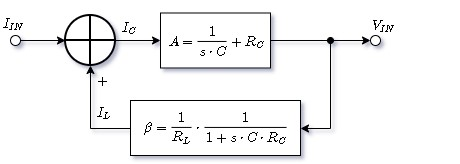
\includegraphics[scale=0.7]{../EJ2/Recursos/sistema_gyrator.jpg}
    \caption{Sistema a lazo cerrado del circuito Gyrator propuesto}
    \label{fig:sistema_gyrator}
\end{figure}

Se caracteriza la funci\'on transferencia, es decir la impedancia de entrada del circuito, en t\'erminos generales se llega a que:

\begin{equation}
    Z_{IN}(s) = \frac{A}{1 + \beta \cdot A}
\end{equation}

Particularmente para los casos donde, como suele suceder con los sistemas a lazo cerrado, la magnitud de $A >> 1$, entonces se puede aproximar
la funci\'on como:

\begin{equation}
    Z_{IN}(s) \approx \frac{1}{\beta} = R_L + s \cdot C \cdot R_C \cdot R_L
\end{equation}

Desde este punto de vista, para tales condiciones el circuito se comporta como una bobina, lo cual coincide con el an\'alisis puramente circuital. 

\subsection{Filtro Pasabajos}

\subsubsection{Dise\~no de funci\'on transferencia}
Consid\'erese un sistema de segundo orden lineal, de tiempo invariante y bibo-estable, en cuyo caso analizar la funci\'on transferencia que caracteriza a un sistema
que se comporta como un filtro pasabajos tiene una forma gen\'erica dada como se muestra en la Ec. \ref{eq:funcion_pasabajos}.

\begin{equation}
    H(s) = \frac{V_o(s)}{V_i(s)} = \frac{1}{1 + \frac{s}{\omega_o \cdot Q} + \left( \frac{s}{\omega_o}\right)^{2}}
    \label{eq:funcion_pasabajos}
\end{equation}

Se elige una funci\'on transferencia de esta forma porque al tener \'unicamente polos, salvo en la regi\'on de la banda pasante, el circuito atenuar\'a las altas frecuencias por la ca\'ida causada por los polos. En un principio el sistema propuesto
puede estar dado como un subamortiguado, cr\'iticamente amortiguado o un sobreamortiguado. Se descarta la posibilidad de que se encuentre subamortiguado ya que presentar\'ia un sobrepico en un entorno de la frecuencia de corte
que modificar\'ia el comportamiento buscado, por otro lado se busca que idealmente sea un cr\'iticamente amortiguado porque de esa forma tiene una pendiente de decrecimiento mayor. Para tal caso, el sistema presenta dos polos reales e iguales, ubicados en $\omega_o$. De esta forma se reduce la expresi\'on a la forma:

\begin{equation}
    H(s) = \frac{1}{\left(1 + \frac{s}{\omega_o}\right)^{2}}
    \label{eq:funcion_pasabajos_ideal}
\end{equation}

Como se busca que esta funci\'on cumpla con las condiciones de la plantilla inicialmente presentada al comienzo de esta secci\'on, luego se eval\'ua para tales frecuencias
y se obtienen condiciones sobre c\'omo debe ser el valor de la frecuencia de corte para lograr cumplir con los requisitos. En las frecuencias de corte los l\'imites est\'an dados respectivamente por
$-3dB$ y $-10dB$, sin embargo para tener m\'as margen de error, se acota a que est\'e en $-2dB$ y en $-11dB$.

\begin{eqnarray*}
    & |H(\omega_p)|dB \geq -2dB \Rightarrow 20 \cdot \log{\left(\frac{1}{1 + \left(\frac{\omega_p}{\omega_o}\right)^{2}}\right)} \geq -2dB\\
    & \Rightarrow \omega_o \geq 2\pi \cdot 5.9kHz
\end{eqnarray*}

\begin{eqnarray*}
    & |H(\omega_a)|dB \leq -11dB \Rightarrow 20 \cdot \log{\left(\frac{1}{1 + \left(\frac{\omega_a}{\omega_o}\right)^{2}}\right)} \leq -11dB \\
    & \Rightarrow \omega_o \leq 2 \pi \cdot 6.57kHz
\end{eqnarray*}

Por lo tanto, si se ubica la frecuencia de corte dentro del rango $5.9kHz < f_o < 6.57kHz$ luego se puede garantizar que se cumple con la plantilla. Si se lo ubica en el valor medio del rango,
se logra que ante cualquier variaci\'on por la dispersi\'on de las caracter\'isticas de los componentes tenga el mayor marge de forma sim\'etrica. 
Entonces $f_o = \frac{5.9kHz + 6.57kHz}{2} = 6.235kHz$. Desde este punto de vista, la m\'axima variaci\'on para la frecuencia de corte sin que se salga de lo requerido,
est\'a dado como $\Delta f = \frac{6.57kHz - 5.9kHz}{2} = 370Hz$, por lo tanto la frecuencia de corte puede desviarse un $5\%$ aproximadamente. Lo cual si bien no es tan amplio como se quisiera, hay que recordar
que se parten de sobredimensionamientos iniciales, con lo cual salirse un poco de dicho margen no deber\'ia implicar un riesgo, pero aumenta la probabilidad de que el resultado sea el esperado mantenerse en tal regi\'on acotada.

\subsubsection{Dise\~no de circuito con Gyrator}
Desde un punto de vista matem\'atico se encontr\'o que la Ec. \ref{eq:funcion_pasabajos_ideal} describe un sistema que se comporta como un filtro pasabajos que dentro de ciertas condiciones
acotadas de variaci\'on de los par\'ametros, logra cumplir con los requerimientos de la plantilla del filtro. Con lo cual ahora el objetivo es lograr dise\~nar un circuito que permita implementar
pr\'acticamente tal funci\'on transferencia.

En general, en el dise\~no de filtros an\'alogicos pasivos se utilizar\'ia un circuito RLC y si se analiza la diferencia de potencial sobre el capacitor, se ver\'ia un filtro pasabajos que podr\'ia llegar a utilizarse
para poder implementar la funci\'on ideal encontrada. No obstante, como bien se mencion\'o con anterioridad, en la pr\'actica para bajas frecuencias no suele utilizarse un inductor por su tama\~no y limitado rango de funcionamiento,
adem\'as de los efectos par\'asitos que suele traer consigo. Por esto mismo, se utilizar\'a el circuito Gyrator.


En rasgos generales, el proceso de dise\~no consiste inicialmente en proponer una configuraci\'on con el circuito Gyrator con la cual pueda llegarse a una funci\'on transferencia deseada,
luego utilizando un an\'alisis ideal determinar los valores de componentes y, finalmente, realizar un an\'anisis no ideal menos aproximado para determinar condiciones de operaci\'on o limitaciones sobre
el amplificador operacional, para que se cumpla lo mayor posible el resultado ideal.

\paragraph*{Circuito equivalente aproximado:} Considerando que con un Gyrator bajo ciertas condiciones se puede simular un inductor con una resistencia en serie, si se agrega un capacitor adicional puede armarse un simple circuito RLC para el filtro,
por tanto se analiza el circuito que se ilustra en la Fig. \ref{fig:equivalente_gyrator}. Consid\'erese que en la determinaci\'on de los valores de componentes se establecer\'a $R_L >> R_G$ con lo cual el efecto de 
la resistencia del generador puede despreciarse y no produce una desviaci\'on notable. 

\begin{figure}[H]
    \centering
    \includegraphics[scale=0.6]{../EJ2/Recursos/equivalente_pasabajos.png}
    \caption{Circuito pasabajos equivalente}
    \label{fig:equivalente_pasabajos}
\end{figure}

\begin{eqnarray*}
    & H(s) = \frac{V_o(s)}{V_i(s)} = \frac{ \frac{1}{s \cdot C_2} }{ s \cdot L + R_L + \frac{1}{s \cdot C_2}} = \frac{1}{s^{2} \cdot L \cdot C + s \cdot C_2 \cdot R_L + 1} \\
    & \Rightarrow \omega_o = \frac{1}{\sqrt{(LC)}} \Rightarrow L = \frac{1}{C_2 \cdot (2\pi \cdot 6.235kHz)^{2}} \\
    & \Rightarrow \xi = 1 \rightarrow C_2 \cdot R_L = \frac{2}{\omega_o} \Rightarrow R_L = \frac{1}{\pi \cdot 6.235kHz \cdot C_2}
\end{eqnarray*}

Parametrizando los valores de componentes en funci\'on del capacitor de salida, luego se puede determinar un valor de capacidad el cual sea lo suficientemente grande para que no se vea afectado
por capacidades par\'asitas o capacidades correspondientes a las puntas de medici\'on del osciloscopio, con lo cual utilizando $C_2 = 33nF$ luego se obtiene que $R_L = 1.5k \Omega$ y $L = 19.74mH$.

\paragraph*{Circuito completo:} En la Fig. \ref{fig:circuito_gyrator} se ilustra el esquema completo del circuito implementado con un Gyrator, para lo cual como inicialmente se hizo el an\'alisis considerando que el inductor no era flotante sino que estaba conectado a la masa del circuito,
se emplea esta conexi\'on donde se logra establecer que la impedancia de salida o de thevenin vista por el capacitor se corresponda efectivamente a analizar que cuando se pasiva $V_i$, entonces se obtiene nuevamente lo que se estudi\'o previamente del Gyrator. Con lo cual ahora se deben dimensionar los componentes
del Gyrator para que se corresponda el funcionamiento equivalente antes estudiado.

Para realizar esto se reutilizan las expresiones obtenidas al estudiar el Gyrator en las primeras secciones, donde se obten\'ia una condici\'on de funcionamiento y la ecuaci\'on para determinar la inductancia.
La condici\'on estaba dada por el hecho de que se defin\'ia una frecuencia angular $\omega_o = \frac{1}{C \cdot R_L}$ y se estableci\'o que el comportamiento inductivo se dar\'ia siempre y cuando $\omega << \omega_o$, esto quiere decir que no siempre
se mantendr\'a el comportamiento equivalente, pero como se comporta como un filtro pasabajos es de inter\'es que \'unicamente se sostenga al menos para el rango de frecuencias en las cuales se eval\'uan los criterios establecidos. Por ende,
se pide que $f_o \geq 10 \cdot f_a = 100,5kHz$.

\begin{eqnarray}
    & C_{max} = \frac{1}{\omega_{o_{min}} \cdot R_L} = \frac{1}{1.5k \Omega \cdot 2\pi \cdot 100.5kHz} = 1.05nF\\
    & R = \frac{1}{C \cdot R_L} \Rightarrow C = 470pF \rightarrow R = 28k \Omega = 56k\Omega // 56k\Omega
\end{eqnarray}

\begin{figure}[H]
    \centering
    \includegraphics[scale=0.5]{../EJ2/Recursos/circuito_pasabajos.png}
    \caption{Circuito completo pasabajos con Gyrator}
    \label{fig:circuito_pasabajos}
\end{figure}

\paragraph*{An\'alisis no ideal:} Considerando que el amplificador operacional tiene un funcionamiento no ideal, esto es, con un $A_{vol}$ finito y con un polo dominante
a partir del cual decrece tal magnitud, y llamando como $V_A$ al potencial en la salida de dicho amplificador, luego se realiza un an\'alisis planteando las siguientes ecuaciones
sobre el circuito, de las cuales desarroll\'andolas se obtiene finalmente una expresi\'on para la transferencia del circuito sin aproximaciones ni idealidades.

\begin{align}
    & V^{-} = V_A \\
    & V^{+} = \frac{V_i + s \cdot C \cdot R \cdot V_o}{1 + s \cdot C \cdot R} \\
    & I_{C} + I_{R_L} = I_{C_2} \Rightarrow \frac{(V_i - V_o) \cdot s \cdot C}{1 + s \cdot C \cdot R} + \frac{V_A - V_o}{R_L} = s \cdot C_2 \cdot V_o \\
    & V_A = (V^{+} - V^{-}) \cdot A_{vol} \\
    & A_{vol} = \frac{A_o}{1 + \frac{s}{\omega_p}}
\end{align}

El siguiente desarrollo final obtenido ya tiene como aproximaciones algunas consideraciones como considerar que $A_o + 1 \approx A_o$.

\begin{align}
    & H(s) \approx \frac{1}{1 + \frac{s}{GBP}} \cdot \frac{1 + \frac{s}{\omega_1} + \frac{s^{2}}{GBP \cdot \omega_1}}{1 + s \cdot \beta + s^{2} \cdot \alpha} \\
    & \alpha = C \cdot R \cdot C_2 \cdot R_L \\
    & \beta = C_2 \cdot R_L + C \cdot R_L \\
    & \omega_1 = \frac{1}{C \cdot R_L} \\
    & GBP = \omega_p \cdot A_o
\end{align}

Entonces, con esta nueva expresi\'on que inicialmente dista en comportamiento de lo que se desea, se empiezan a aplicar criterios que permitan demostrar que para una regi\'on limitada del espectro de frecuencias,
el comportamiento ser\'a el inicialmente planteado. En primer lugar, en el an\'alisis ideal ya se tuvo en cuenta que $\omega << \omega_1$ para la operaci\'on del filtro, con lo cual el t\'ermino lineal del numerador puede despreciarse respecto del 
t\'ermino independiente, aunque por otro lado queremos que lo mismo suceda para el t\'ermino cuadr\'atico del numerador con lo cual es necesario que se cumpla como condici\'on que $\omega << \sqrt{GBP \cdot \omega_1}$ y nuevamente como se hizo antes,
se toma como referencia que esto valga al menos para las frecuencias de referencia donde opera el pasabajos, entonces se pide que $\sqrt{GBP \cdot \omega_1} \geq 10 \cdot 2\pi \cdot 10.5kHz$.
Por otro lado, aparece un polo adicional para el cual solo basta pedir que el valor de $GBP >> \omega$ para los rangos de funcionamientos deseados.

\begin{align*}
    & GBP \geq \frac{(2\pi \cdot 105kHz)^{2}}{\omega_1} = 2\pi \cdot 48.83kHz \\
    & GBP \geq 2\pi \cdot 105kHz
\end{align*}

Entonces, se puede aproximar correspondiente que:

\begin{equation}
    H(s) \approx \frac{1}{1 + s \cdot \beta + s^{2} \cdot \alpha}
\end{equation}

\subsubsection{Verificaci\'on del dise\~no}
Para el armado del circuito en la pr\'actica se utilizar\'an resistencias de una tolerancia de $1\%$, y capacitores con una tolerancia de $10\%$, esto provoca que en la realidad
pueda haber una dispersi\'on que modifique el resultado final del filtro. Para conocer la posible variaci\'on y asegurar que est\'e dentro de un rango aceptable, se simula en LTSpice
y obtiene la respuesta en frecuencia usando Monte Carlo para variar los componentes. S\'olo se ilustra el m\'odulo del resultado porque no es de inter\'es la fase a los prop\'ositos de estas observaciones. 
Los resultados pueden observarse en las figuras mostradas en \ref{fig:lp_montecarlo} y \ref{fig:lp_montecarlo_frecuencias} y puede observarse que para las frecuencias pasante y atenuante se cumple con los criterios
adoptados en el dise\~no.

\begin{figure}[H]
    \centering
    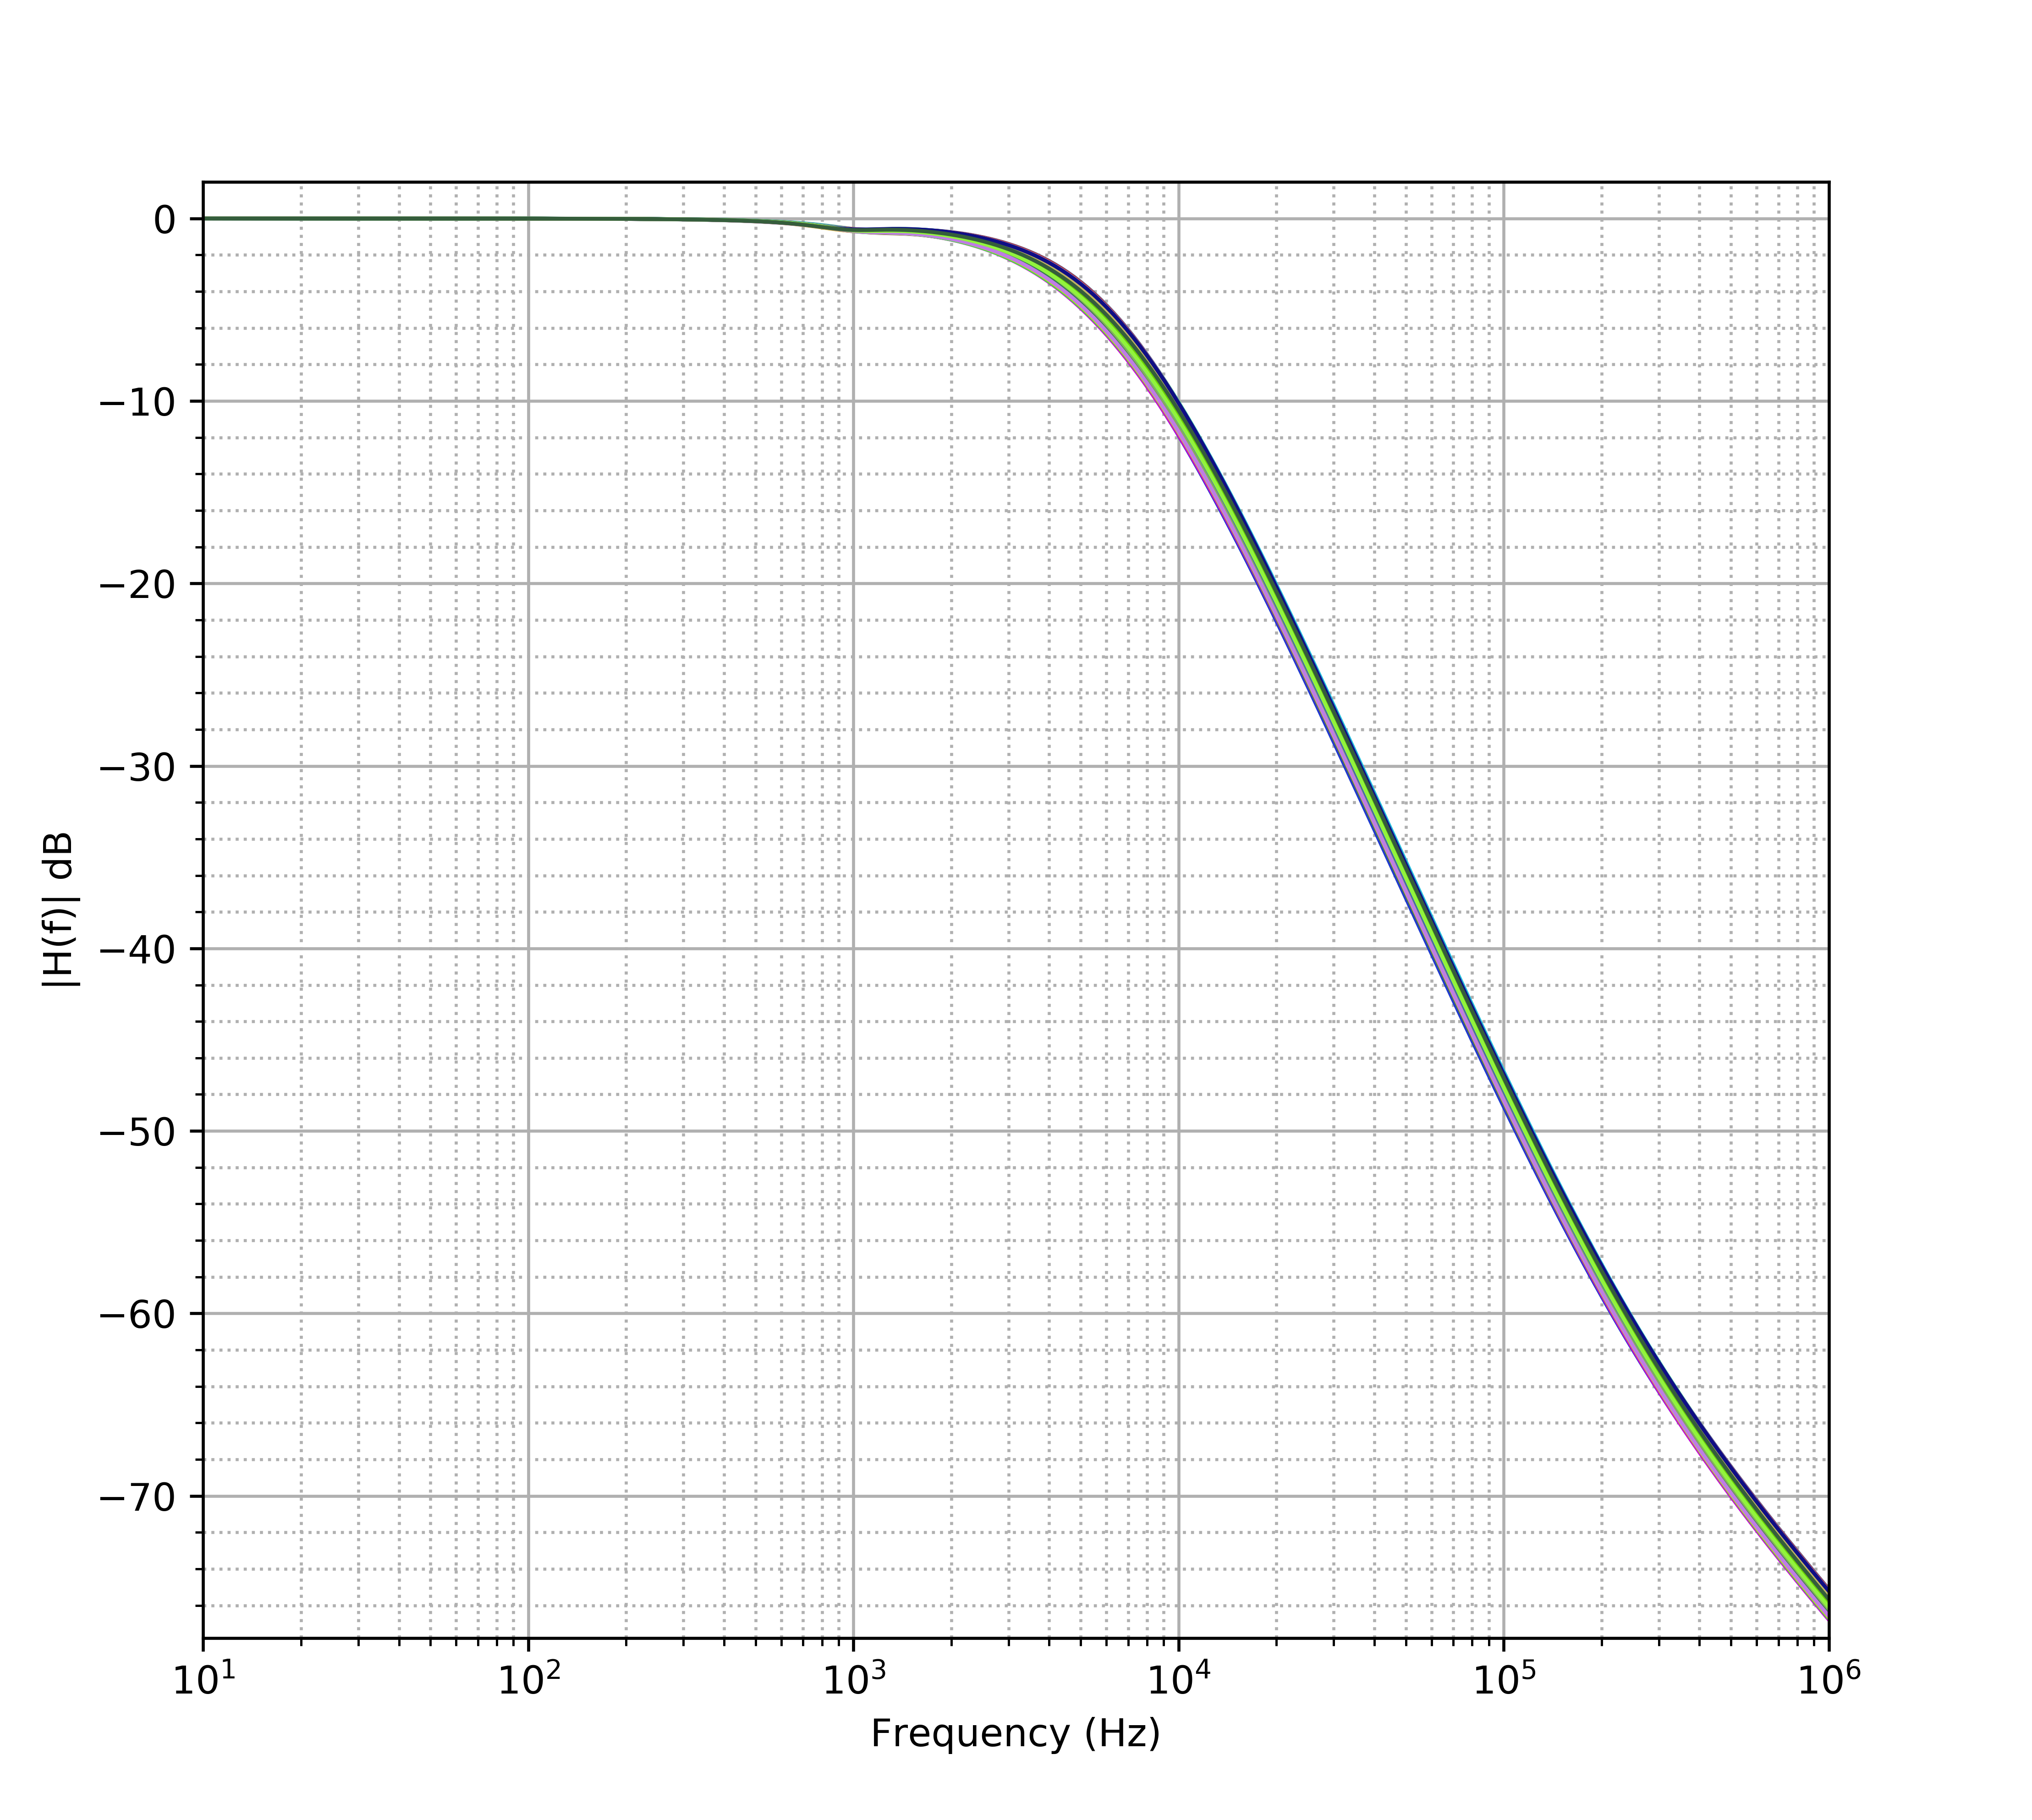
\includegraphics[scale=0.12]{../EJ2/Recursos/lp_montecarlo.png}
    \caption{M\'odulo de la respuesta en frecuencia del filtro pasabajos en escala semilogar\'itmica}
    \label{fig:lp_montecarlo}
\end{figure}

\begin{figure}[H]
    \centering
    \begin{tabular}{c c}
        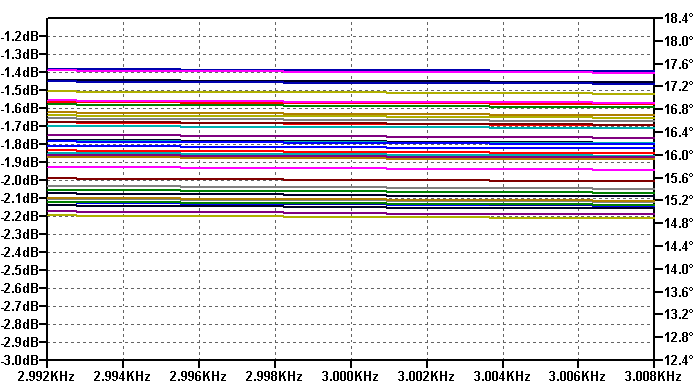
\includegraphics[scale=0.4]{../EJ2/Recursos/lp_montecarlo_fp.png}
        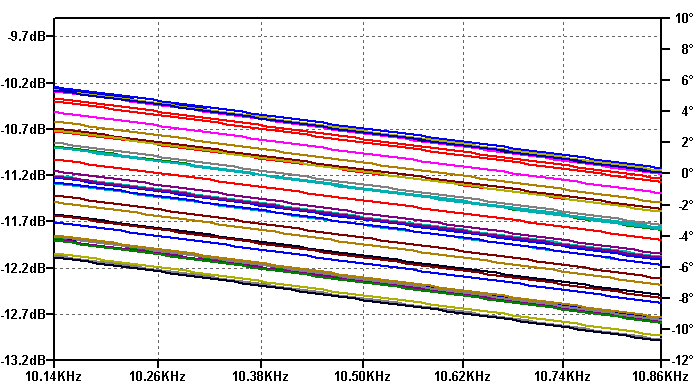
\includegraphics[scale=0.4]{../EJ2/Recursos/lp_montecarlo_fa.png}
    \end{tabular}
    \caption{Vista aumentada en frecuencias pasante y atenuante}
    \label{fig:lp_montecarlo_frecuencias}
\end{figure}

\subsubsection{Resultados}

\subsection{Filtro Pasaaltos}

\subsubsection{Dise\~no de funci\'on transferencia}
Consid\'erese un sistema de segundo orden lineal, de tiempo invariante y bibo-estable, tal que describe un comportamiento
pasaaltos, esto es, que aten\'ua aquellas se\~nales de entrada con frecuencia menor respecto de una referencia denominada frecuencia de corte.
Para esto \'ultimo, se propone una funci\'on transferencia que modeliza matem\'aticamente este sistema, expresada en la Ec. \ref{eq:funcion_pasaaltos}.

\begin{equation}
    H(s) = \frac{ \frac{s^{2}}{\omega_o^{2}} }{\left(\frac{s}{\omega_o}\right)^{2} + s \cdot \frac{2 \cdot \xi}{\omega_o} + 1}
\end{equation}

La funci\'on transferencia caracteriza un sistema de segundo orden el cual se puede encontrar en tres diferentes condiciones, sea subamortiguado, sobreamortiguado o cr\'iticamente amortiguado,
para lo cual se descarta la primera posibilidad ya que provocar\'ia la aparici\'on de un sobrepico en el entorno de la frecuencia de corte, modificando la respuesta deseada. Por otro lado, se desea que el resultado
sea lo m\'as comparable con un filtro ideal, con lo cual para simular el cambio m\'as abrupto posible se busca que sea cr\'ticamente amortiguado para tener la mayor pendiente posible de decrecimiento, para el orden dado.
Esto \'ultimo implica que se condiciona al sistema a tener un valor de $\xi = 1$.

\begin{equation}
    H(s) = \frac{\left(\frac{s}{\omega_o}\right)^{2}}{\left(\frac{s}{\omega_o} + 1\right)^{2}}
    \label{eq:funcion_pasaaltos}
\end{equation}

Luego es necesario determinar la frecuencia de corte de dicho filtro. Para determinar este valor se toma como condici\'on de dise\~no cumplir con la plantilla presentada al inicio de la secci\'on, con lo cual
se eval\'ua la magnitud de la respuesta en frecuencia para las dos frecuencias de referencia y se imponen condiciones tomando un determinado margen de error.

\begin{eqnarray*}
    & |H(\omega_p)|dB > -2dB \Rightarrow 20 \cdot \log{\left( \frac{\frac{\omega_p^{2}}{\omega_o^{2}}}{1 + \frac{\omega_p^{2}}{\omega_o^{2}}} \right)} \\
    & \Rightarrow \omega_o < 2\pi \cdot 1.78kHz 
\end{eqnarray*}

\begin{eqnarray*}
    & |H(\omega_a)|dB < -11dB \Rightarrow 20 \cdot \log{ \left(  \frac{\frac{\omega_a^{2}}{\omega_o^{2}}}{1 + \frac{\omega_a^{2}}{\omega_o^{2}}} \right) } \\
    & \Rightarrow \omega_o > 2\pi \cdot 1.596kHz
\end{eqnarray*}

A partir de esto se puede considerar que siempre y cuando la frecuencia de corte que limite a quedar acotada dentro del rango $1.59kHz < f_o < 1.78kHz$ luego se cumplir\'an
las condiciones de dise\~no que fueron impuestas sobre el sistema. En caso de variar el valor de tal frecuencia, lo mejor es tomar como valor nominal el punto medio del rango, para tener la m\'axima
variaci\'on posible de forma sim\'etrico, con lo cual se escoge $f_o = 1.688kHz$. Con esta apreciaci\'on se puede ver que la variaci\'on de tal frecuencia que se permite es, porcentualmente,
un $5.4\%$.

\subsubsection{Dise\~no de circuito con Gyrator}

En un principio para poder implementar en un circuito un filtro pasaaltos descripto por la Ec. \ref{eq:funcion_pasaaltos} podr\'ia utilizarse una configuraci\'on RLC determinada,
con lo cual si se posee un Gyrator que ya de por s\'i corresponde equivalentemente a una inductor con una resistencia en serie, en principio se podr\'ia asumir que agregando un capacitor en serie ya es suficiente.
Esto fue lo que se intento hacer con el circuito equivalente de la Fig. \ref{fig:equivalente_pasaaltos_fallido}, consid\'erese el sistema recuadradao como el que se analiza sin considerar la impedancia del generador dado
que no puede incluirse dentro de las mediciones.

\begin{figure}[H]
    \centering
    \includegraphics[scale=0.5]{../EJ2/Recursos/equivalente_pasaaltos_fallido.png}
    \caption{Circuito equvalente fallido}
    \label{fig:equivalente_pasaaltos_fallido}
\end{figure}

\begin{equation*}
    H(s) = \frac{s^{2} \cdot LC \cdot (1 + \frac{R_L}{s \cdot L})}{s^{2} \cdot LC + s \cdot C \cdot R_L + 1}
    \label{eq:funcion_pasaaltos_fallida}
\end{equation*}

El problema de este circuito o esta configuraci\'on propuesta se refleja en la Ec. \ref{eq:funcion_pasaaltos_fallida}, si se observa con atenci\'on difiere con respecto a la que idealmente se dise\~no por un factor
adicional en el numerador, esto se debe a la presencia de la resistencia $R_L$ en la rama de salida y lo que ser\'ia beneficioso a los fines de este an\'alisis ser\'ia poder despreciar el efecto de tal factor en la funci\'on, no obstante para ello
habr\'ia que plantear $\frac{R_L}{\omega \cdot L} << 1 \Rightarrow \frac{R_L}{L} << \omega$. Es ac\'a donde esta propuesta falla en el sentido en que su comportamiento se va a desviar mucho de lo buscado,
ya que ese t\'ermino muy dif\'ilmente cumpla tal condici\'on, y se puede ver si se plantean las condiciones sobre $R_L$ y $L$ para cumplir inicialmente con el valor de $\xi$ y de $\omega_o$ del sistema.

\begin{align*}
    & L = \frac{1}{(2 \pi \cdot f_o)^{2} \cdot C} \\
    & R_L = \frac{1}{\pi \cdot f_o \cdot C} \\
    & \Rightarrow \frac{R_L}{L} = 4 \pi \cdot f_o
\end{align*}

Esto quiere decir que para las frecuencias de inter\'es, ya sean las de referencia para el filtro o la de corte, el factor tendr\'a un efecto apreciable que modificar\'a
su comportamiento resultante. 

\paragraph*{Circuito equivalente aproximado:} Para solucionar esto, se propone una nueva forma del circuito, agregando una resistencia en serie al capacitor como se puede observar en la Fig. \ref{fig:equivalente_pasaaltos}.

\begin{figure}[H]
    \centering
    \includegraphics[scale=0.6]{../EJ2/Recursos/equivalente_pasaaltos.png}
    \caption{Circuito equivalente del filtro pasaaltos}
    \label{fig:equivalente_pasaaltos}
\end{figure}

En primer lugar, si bien el sistema a analizar es el que comienza posterior a la resistencia del generador, es importante tener en cuenta su valor y buscar que la resistencia
$R$ sea mucho m\'as grande para que las desviaciones al sistema por la presencia de $R_G$ sean m\'inimas, es decir, que se cumpla que $R_G << R$. De esta forma la resistencia total
del circuito RLC no se desviar\'a mucho del valor esperado para el caso amortiguado que se busca. Con esto en mente, se desarrolla y se llega a que la funci\'on transferencia est\'a dada:

\begin{align}
    & H(s) = \frac{s^{2} \cdot LC \cdot (1 + \frac{R_L}{s \cdot L})}{1 + s \cdot C \cdot (R_L + R) + s^{2} \cdot LC} \\
    & \xi = 1 \Rightarrow R + R_L = \frac{1}{\pi \cdot f_o \cdot C} = \frac{1}{\pi \cdot 1.688kHz \cdot C}\\
    & L = \frac{1}{(2 \pi \cdot f_o)^{2} \cdot C} = \frac{1}{(2 \pi \cdot 1.688kHz)^{2} \cdot C}
\end{align}

Nuevamente en este circuito se puede ver que hay un factor en el numerador que en la expresi\'on ideal no se encuentra, con lo cual se busca despreciar sus efectos. Para lograr esto, y de la misma forma que se analiz\'o en el caso del circuito fallido,
se debe imponer que se cumpla que $\frac{R_L}{L} << \omega$. Esta vez esto es posible, el por qu\'e se atribuye a que la presencia de una nueva resistencia en el circuito influye en el valor del coeficiente de amortiguamiento con lo cual no est\'a determinado
el valor de $R_L$ y este nuevo grado de libertad permite dividir los requisitos entre las resistencias. Se propone considerar que la frecuencia por debajo de la cual deberia volverse apreciable tal factor est\'e debajo de $f \approx 100Hz$ por considerar una d\'ecada
de separaci\'on con la primer frecuencia de referencia y evitar las desviaciones pertinentes. Entonces adem\'as se impone $R_L << 2\pi \cdot 100Hz \cdot L$.

Se propone un valor de capacidad $C = 33nF$, con lo cual la inductancia tiene que tener un valor de $L = 269.39mH$. Consecuentemente, la resistencia $R_L < 169.26 \Omega$, y luego la suma de ambas resistencia
tiene un valor de $R + R_L = 5714.3 \Omega$, por lo cual se toma $R_L = 120 \Omega$ y $R = 5.6k\Omega$. Si se tiene en cuenta que para la implementaci\'on pr\'actica de estos circuitos se utilizar\'an resistencia SMD
de potencia nominal 1/8W, resulta necesaria hacer una menci\'on sobre el valor bajo de $R_L$ y analizar la posibilidad de que implica una potencia disipada mayor. No obstante, como esta resistencia en el circuito equivalente se encuentre en la rama de 
salida en serie con la inductancia, para las frecuencias bajas en las cuales tal resistencia sea comparable con la magnitud de la impedancia del inductor, luego la salida se ver\'a atenuada demasiado como para producir una ca\'ida de tensi\'on que genere disipaci\'on
por encima de lo nominal, por otro lado, en las condiciones en las cuales la salida no se ve atenuada luego la impedancia del inductor crece en magnitud y la proporci\'on sobre la resistencia disminuye, con lo cual al igual que antes tampoco puede producir una disipaci\'on notable.

\paragraph*{Circuito completo:} En la Fig. \ref{fig:circuito_pasaaltos} se puede observar el esquema completo del circuito implementando la bobina, es decir el inductor con una resistencia en serie, empleando para ello un Gyrator.
Es necesario por ende determinar los valores del circuito para que simule efectivamente al inductor, para lo cual se parte inicialmente de una condici\'on, donde se pide que $\frac{1}{C_2 \cdot R_L} > 2 \pi \cdot 500kHz$. Esto \'ultimo es para alejar los efectos no deseados del Gyrator, despreciandolos
y considerando que para frecuencias bajas del filtro luego se comporte como inductor, no obstante el valor dado de frecuencia es una elecci\'on arbitraria. Por otro lado, a partir de tal consideraci\'on se propone $C_2 = 2.7nF$ y se obtiene que como $L = R_L \cdot C_2 \cdot R_C$, entonces $R_C = 820k\Omega$.

\begin{figure}[H]
    \centering
    \includegraphics[scale=0.55]{../EJ2/Recursos/circuito_pasaaltos.png}
    \caption{Circuito completo del pasaaltos}
    \label{fig:circuito_pasaaltos}
\end{figure}

\paragraph*{An\'alisis no ideal:} Si se considera un amplificador operacional no ideal, esto es, con un $A_{vol}$ finito y con polo dominante, luego adem\'as
se considera que la corriente de entrada es despreciable, entonces planteando diferentes ecuaciones para caracterizar al circuito se puede llegar a la funci\'on transferencia
del mismo.

\begin{align}
    & V^{+} = \frac{V_o \cdot s \cdot C_2 \cdot R_C}{1 + s \cdot C_2 \cdot R_C} \\
    & V^{-} = V_A \\
    & V_A = (V^{+} - V^{-}) \cdot A_{vol} \\
    & A_{vol} = \frac{A_o \cdot \omega_p}{s + \omega_p} = \frac{GBP}{s + \omega_p} \\
    & I_{C} = I_{C_2} + I_{R_L} \Rightarrow \frac{(V_i - V_o) \cdot s \cdot C}{1 + s \cdot C \cdot R} = \frac{V_o \cdot s \cdot C_2}{1 + s \cdot C_2 \cdot R_C} + \frac{V_o - V_A}{R_L}
\end{align}

Luego si se considera como condici\'on de la selecci\'on del amplificador operacional, se que cumpla que para las frecuencias de trabajo luego $\omega << GBP$, entonces se puede aproximar
al siguiente resultado inicial la funci\'on transferencia.

\begin{align}
    H(s) = \frac{s \cdot C \cdot R_L \cdot (1 + s \cdot C_2 \cdot R_C)}{s^{2} \cdot C_2 \cdot C \cdot R_C \cdot R_L \cdot (1 + \frac{R}{R_C}) + s \cdot C \cdot (R + R_L) + s \cdot C_2 \cdot R_L + 1}    
\end{align}

Luego si se cumple para el numerador que la expresi\'on dada por $1 + s \cdot C_2 \cdot R_C \approx s \cdot C_2 \cdot R_C$, con lo cual para ello debe suceder que en las frecuencias de trabajo
se pueda considerar que $\omega >> \frac{1}{C_2 \cdot R_C}$. Por otro lado, para el denominador es necesario considerar que $R >> R_C$ y que, como bien se plante\'o dentro de los criterios tomados para el Gyrator, que $\omega << \frac{1}{C_2 \cdot R_L}$, teniendo en mente
estos criterios de dise\~no, se puede aproximar luego la funci\'on transferencia a la siguiente forma.

\begin{equation}
    H(s) \approx \frac{s^{2} \cdot C_2 \cdot C \cdot R_L \cdot R_C}{s^{2} \cdot C_2 \cdot C \cdot R_C \cdot R_L + s \cdot C \cdot (R + R_L) + 1}
\end{equation}

Usualmente se esperar\'ia que de un an\'alisis no aproximado se obtuvieran condiciones sobre el amplificador operacional principalmente, las cuales si bien se obtuvieron, no fueron tantas como las condiciones
sobre los valores del circuito. Esto \'ultimo es un resultado inesperado que es necesario reconsiderar para verificar que los valores tomados para el dise\~no del circuito son v\'alidos.

\subsubsection{Verificaci\'on del dise\~no}
Se verifica a continuaci\'on el funcionamiento del dise\~no del filtro empleando una herramiento de simulaci\'on LTSpice y graficando usando Monte Carlo para considerar las variaciones
por la dispersi\'on de los componentes. Los resultados son ilustrados en las figuras \ref{fig:hp_montecarlo} y \ref{fig:hp_montecarlo_frecuencias}.

\begin{figure}[H]
    \centering
        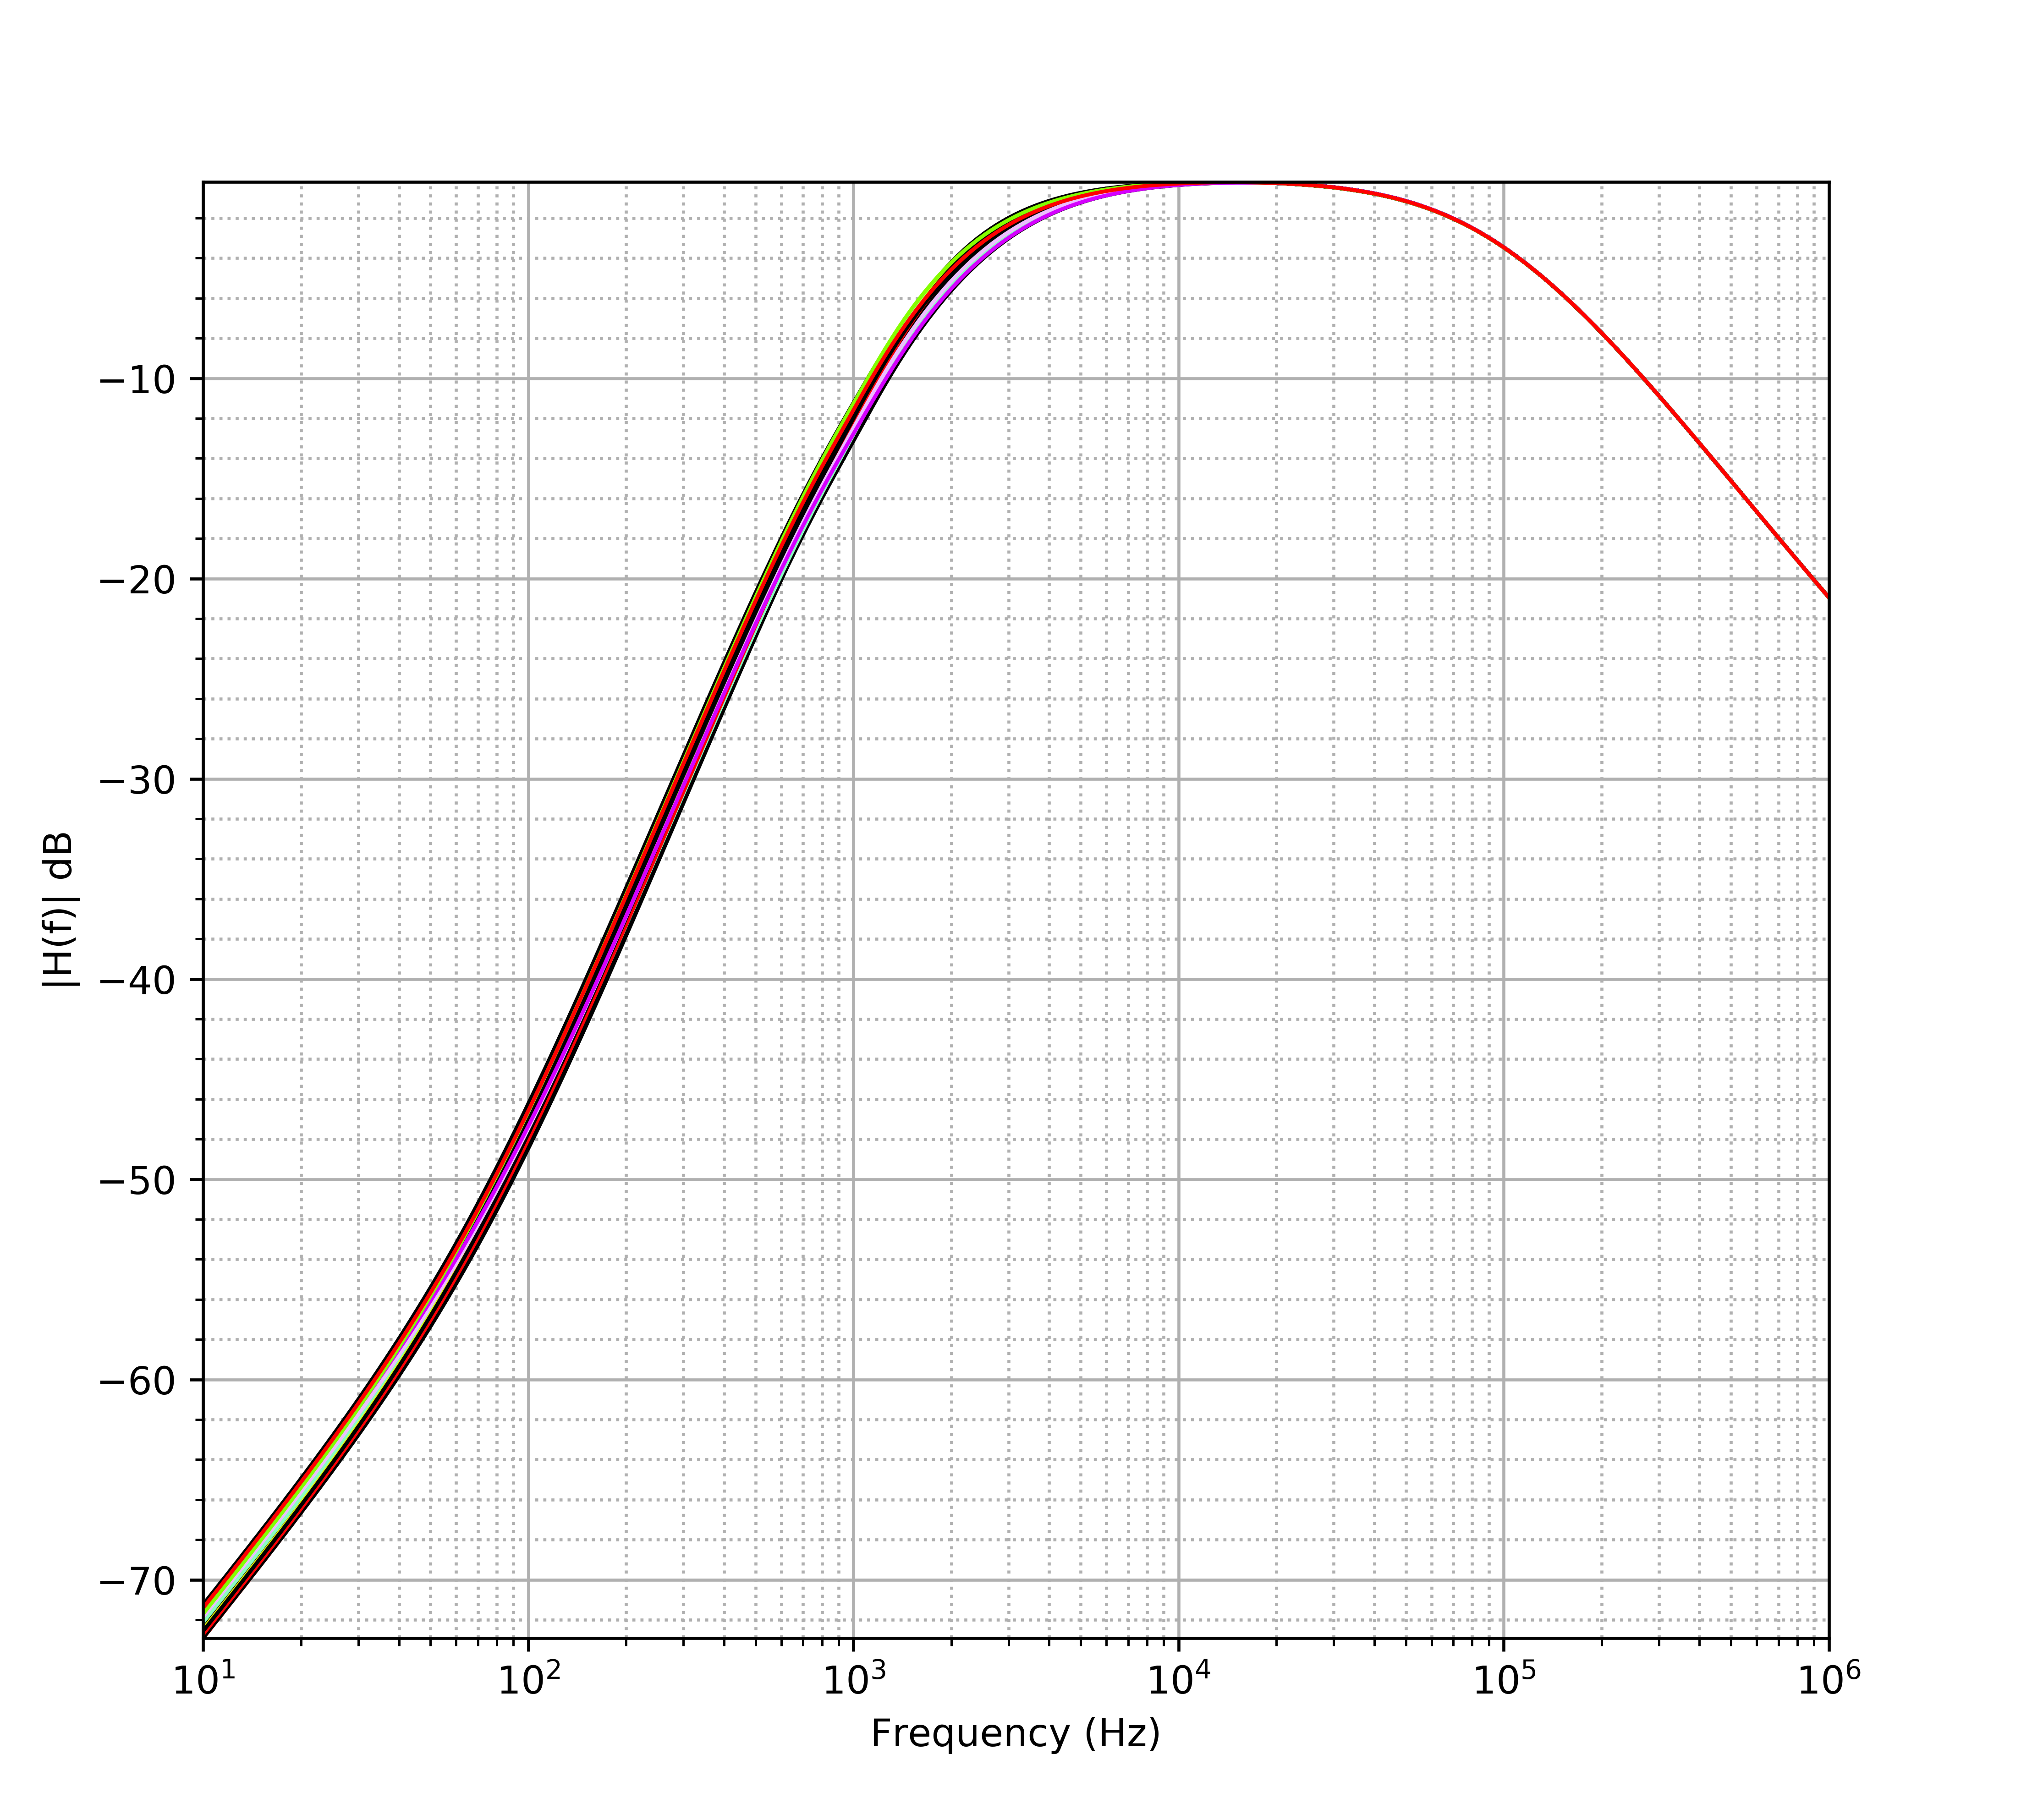
\includegraphics[scale=0.12]{../EJ2/Recursos/hp_montecarlo.png}
    \caption{Respuesta en frecuencia en m\'odulo del filtro pasaaltos}
    \label{fig:hp_montecarlo}
\end{figure}

\begin{figure}[H]
    \centering
    \begin{tabular}{c c}
        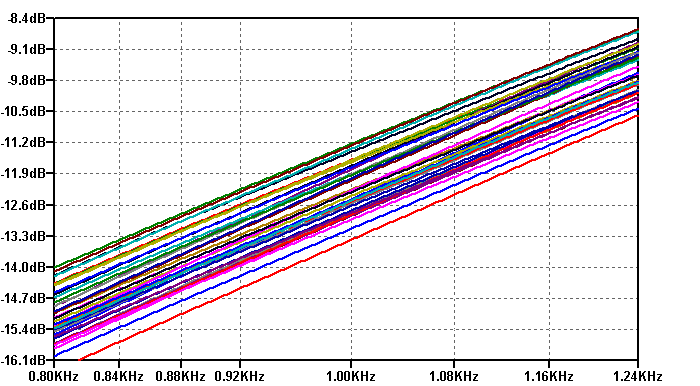
\includegraphics[scale=0.4]{../EJ2/Recursos/hp_montecarlo_fa.png}
        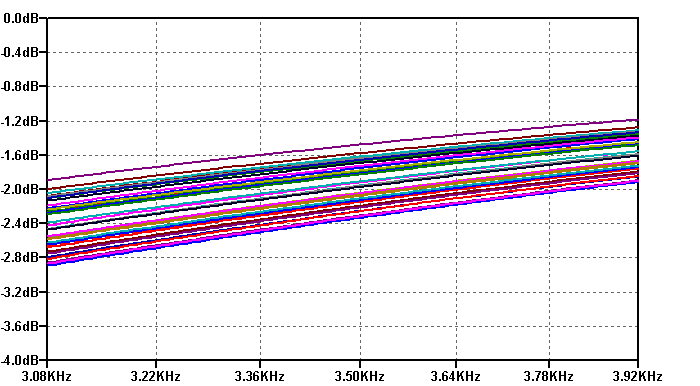
\includegraphics[scale=0.4]{../EJ2/Recursos/hp_montecarlo_fp.png}
    \end{tabular}
    \caption{Acercamiento en frecuencias pasante y atenunante}
    \label{fig:hp_montecarlo_frecuencias}
\end{figure}

\subsubsection{Resultados}

\subsection{Filtro Pasabanda}
\subsubsection{Dise\~no de funci\'on transferencia}
Consid\'erese un sistema de segundo orden lineal, de tiempo invariante y bibo-estable, el cual describe una respuesta en frecuencia caracter\'istica de un sistema pasabanda, esto es,
que aten\'ua a todas aquellas frecuencias que se encuentran fuera del entorno de una frecuencia particular. Para el dise\~no de tal sistema se propone la funci\'on transferencia que lo modela
en la Ec. \ref{eq:funcion_pasabanda}. Se define una constante arbitraria K que depender\'a posteriormente de la implementaci\'on del sistema.

\begin{equation}
    H(s) = \frac{s \cdot K}{\left( \frac{s}{\omega_o} \right)^{2} + \frac{S}{Q \cdot \omega_o} + 1}    
    \label{eq:funcion_pasabanda}
\end{equation}

Espec\'ificamente esta funci\'on transferencia debe atenuar todas aquellas frecuencias fuera del entorno de la $f_o = 6kHz$ seg\'un fue consignado como requisito del filtro, pero adem\'as se impone sobre el circuito
que como pasabanda debe tener un ancho de banda peque\~no que reduzca la extensi\'on del mencionado entorno, para lo cual se busca que el sistema se encuentre subamortiguado. Esto \'ultimo implica que la respuesta en frecuencia poseer\'a
un sobrepico que deber\'a ser ubicado en la frecuencia a filtrar y debe tenerse como cuidado o precauci\'on que no supere los $0dB$. Para lograr ello, se deriva y localiza el extremo absoluto de la funci\'on $|H(w)|$.

\begin{align*}
    & \frac{\delta |H(w)|}{\delta \omega} = 0 \Leftrightarrow \\
    & K \cdot \left[ (\omega_o^{2} - \omega^{2})^{2} + (\frac{\omega_o \cdot \omega}{Q})^{2} \right]
    = \frac{K \cdot \omega}{2} \cdot \left[ -4 \omega \cdot ( \omega_o^{2} - \omega^{2}) + \frac{\omega_o^{2} \cdot \omega \cdot 2}{Q} \right] \Leftrightarrow \\
    & \omega = \omega_o \\
    & |H(\omega_o)| = K \cdot Q \cdot \omega_o
\end{align*}

Por lo tanto, se impondr\'a al sistema que modelice esta expresi\'on matem\'atica, que el valor de $\omega_o = 2\pi \cdot 6kHz$ para cumplir con la frecuencia deseada, y adem\'as,
que cumpla con que $|H(\omega_o)| = K \cdot Q \cdot \omega_o \leq 0dB$.

\subsubsection{Dise\~no de circuito con Gyrator}
De igual forma que para los filtros ya dise\~nados previamente, se seguir\'a un proceso en el cual se dimensarionar\'an los componentes empleandos modelos ideales o aproximados,
determinando los criterios y condiciones donde se logren validar tales comportamientos. No obstante, en el caso de este filtro pasabanda y al igual que puede suceder con muchos circuitos,
existen diferentes alternativas sobre c\'omo implementarlo. Una de las particularidades que tiene este filtro a comparaci\'on del resto es que por filtrar un rango acotado y espec\'ifico de frecuencias,
luego la topolog\'ia del circuito influir\'a mucho sobre la capacidad de establecer con el menor error posible tales frecuencias, por esto mismo es que ante la presencia de dos alternativas, se estudian ambas
evaluando cu\'al de ellas puede llevar consigo mayores ventajas o beneficios.

\paragraph*{Circuito equivalente aproximado:} En un principio se analiza desde un punto de vista aproximado la funci\'on transferencia de ambos circuitos propuestos. El objetivo es comparar ambos comportamientos,
considerar las implicancias, y luego tener en cuenta otros aspectos para determinar la topolog\'ia m\'as conveniente.

\begin{figure}[H]
    \centering
    \begin{tabular}{c c}
        \includegraphics[scale=0.4]{../EJ2/Recursos/equivalente_pasabanda_alternativo.png} & 
        \includegraphics[scale=0.4]{../EJ2/Recursos/equivalente_pasabanda.png}
    \end{tabular}
    \caption{Equivalentes aproximados para el pasabanda, dos alternativas}
    \label{fig:equivalentes_pasabanda}
\end{figure}

Se referir\'a a cada circuito seg\'un el tipo de salida que poseen, por ser una salida con una rama LC o con una rama R, simplemente para facilitar el an\'alisis y las referencias. De esta forma,
en un principio se obtiene la expresi\'on de la funci\'on transferencia para el circuito con salida LC.

\begin{equation}
    H(s) = \frac{s \cdot L + R_L}{s^{2} \cdot L \cdot C \cdot R + s \cdot (C \cdot R \cdot R_L + L) + (R + R_L)}
\end{equation}

Luego para el caso del circuito de salida R.

\begin{equation}
    H(s) = \frac{s \cdot C \cdot R}{s^{2} \cdot L \cdot C + s \cdot C \cdot (R+ R_L) + 1}
\end{equation}

Ambos circuitos poseen una funci\'on transferencia que correctamente configurada puede ser empleada para definir un pasabanda, no obstante en primer lugar para bajas frecuencias el comportamiento es mejor en el circuito de salida R,
ya que en el de salida LC para frecuencias muy bajas la ganancia se mantiene casi constante, aunque podr\'ia ser definida baja y considerarse tal banda atenuada. Esto resulta observable directamente del hecho que la funci\'on $H(s)$ de la salida R
tiene la forma m\'as parecida con el modelo matem\'atico propuesto, ya que posee un cero en el cero.

Por otro lado, en ambos circuitos tanto la inductancia como la capacitancia definen parcialmente la frecuencia de corte, pero en el primer caso de la salida LC adem\'as los valores de las resistencias tambi\'en influyen,
lo cual puede no ser deseado desde dos puntos de vista. En primer lugar, desde un an\'alisis f\'isico, se esperar\'ia que la resonancia de una red compuesta por componentes LC est\'e \'unicamente definida por ellos, variando seg\'un las resistencias
el car\'acter de amortiguamiento. Por otro lado, al haber m\'as componentes que definen una misma variable esto puede implicar que es m\'as sensible en t\'erminos generales a variaciones de todos los componentes.

Finalmente, otro aspecto a comparar es la modulaci\'on de fase que producen a las se\~nales seg\'un la frecuencia estos circuitos. Mientras que el circuito de salida R tiene un comportamiento m\'as acorde a un pasabanda, esto es,
con un decaimiento de $180^{\circ}$, luego el de salida LC tiene una desviaci\'on con respecto a tal comportamiento por la presencia de un cero ubicado en una frecuencia seg\'un la conveniencia del dise\~no.

En conclusi\'on, se opta por el circuito de salida R por las ventajas que conlleva. Para lo cual es necesario aplicar los criterios establecidos previamente en el an\'alisis de la funci\'on transferencia
para determinar la dimensi\'on de los valores de los componentes. Si se considera como condici\'on de dise\~no que la resistencia $R_L$ es al menos diez veces m\'as chica que $R$ y se desprecia su efecto en el t\'ermino
lineal del denominador, luego se puede probar que el valor pico de la respuesta en frecuencia es $|H(\omega_o)| \approx 1$.

\begin{align*}
    & L = \frac{1}{\omega_o^{2} \cdot C} = \frac{1}{(2 \pi \cdot 6kHz )^{2} \cdot C} \\
    & R + R_L = \frac{1}{\omega_o \cdot C \cdot Q}
\end{align*}

Asumiendo un valor de $C = 2.2nF$, luego se obtiene que $L = 0.3198H$ y como se quiere un Q que al menos sea $Q = 1$, entonces como m\'aximo debe suceder que
$R_L + R = 12k\Omega$. Para lo cual se asigna arbitrariamente $R_L = 470 \Omega$ y $R = 10k\Omega$.

\paragraph*{Circuito completo:} en el an\'alisis completo del circuito, considerando las aproximaciones obtenidas a partir del estudio del Gyrator, es necesario definir el valor del capacitor
$C_2$ y de la resistencia $R_C$ del circuito que se ilustra en la Fig. \ref{fig:circuito_pasabanda}. La determinaci\'on de tales valores se hace buscando que la inductancia simulada sea la requerida por la aproximaci\'on previa,
adem\'as de que se cumpla la aproximaci\'on donde $\omega << \frac{1}{C_2 \cdot R_L}$, con lo cual se asignan $C_2 = 6.8nF$ y $100k\Omega$.

\begin{figure}[H]
    \centering
    \includegraphics[scale=0.6]{../EJ2/Recursos/circuito_pasabanda.png}
    \caption{Circuito pasabanda completo con Gyrator}
    \label{fig:circuito_pasabanda}
\end{figure}

\paragraph*{An\'alisis no ideal:} Finalmente, si se considera que en el circuito completo el amplificador operacional no es ideal pues tiene un $A_{vol}$ finito con un polo dominante, luego considerando que la corriente entrante al mismo es despreciable por tener
una gran impedancia de entrada, entonces se plantean ecuaciones para analizar circuitalmente el sistema y luego operando algebraicamente se llega a la soluci\'on final no aproximada. Vale mencionar que se denomina $V_A$ la tensi\'on de salida del amplificador,
y $V_B$ como la tensi\'on entre los dos capacitores $C_2$ y $C$.

\begin{align}
    & V^{-} = V_A \\
    & V^{+} = V_B + \frac{V_i - V_B}{s \cdot C_2 \cdot R_2 + 1} \\
    & A_{vol} = \frac{GBP}{s + \omega_p} \\
    & V_A = (V^{+} - V^{-}) \cdot A_{vol} \\
    & I_{C_2} = I_{R_L} + I_C \Rightarrow \frac{(V_i - V_B) \cdot s \cdot C_2}{1 + s \cdot C_2 \cdot R_2} = \frac{V_B - V_A}{R_L} + \frac{V_B \cdot s \cdot C}{1 + s \cdot C \cdot R}
\end{align}

Entonces, finalmente se obtiene:

\begin{equation}
    H(s) = \frac{s \cdot C \cdot R \cdot (1 + s \cdot C_2 \cdot R_L)}{s^{2} \cdot C_2 \cdot C \cdot R_L \cdot R_2 \cdot (1 + \frac{R}{R_2}) + s \cdot C_2 \cdot R_L + s \cdot C \cdot (R + R_L) + 1}
\end{equation}

En primer lugar, cabe mencionar que para llegar a dicha expresi\'on se consider\'o durante un paso algebraico intermedio que se pod\'ia cumplir para el rango operativo de frecuencias que $\omega << GBP$. Para poder llevar esta expresi\'on a una forma
aproximada donde valga el modelo equivalente que se emple\'o para los dise\~nos, se debe considerar en primer lugar que $R << R_2$, que $R_L << R$ y que $\omega << \frac{1}{C_2 \cdot R_L}$, ya con eso se puede aproximar que:

\begin{equation}
    H(s) \approx \frac{s \cdot C \cdot R}{s^{2} \cdot C \cdot C_2 \cdot R_L \cdot R_2 + s \cdot C \cdot R + 1}
\end{equation}

\subsubsection{Verificaci\'on del dise\~no}
De igual forma que se realiz\'o con los otros filtros, se simula para comprobar el comportamiento de filtro pasabanda y se agrega un an\'alisis de Monte Carlo para poder
contemplar la dispersi\'on por componentes.

\begin{figure}[H]
    \centering
        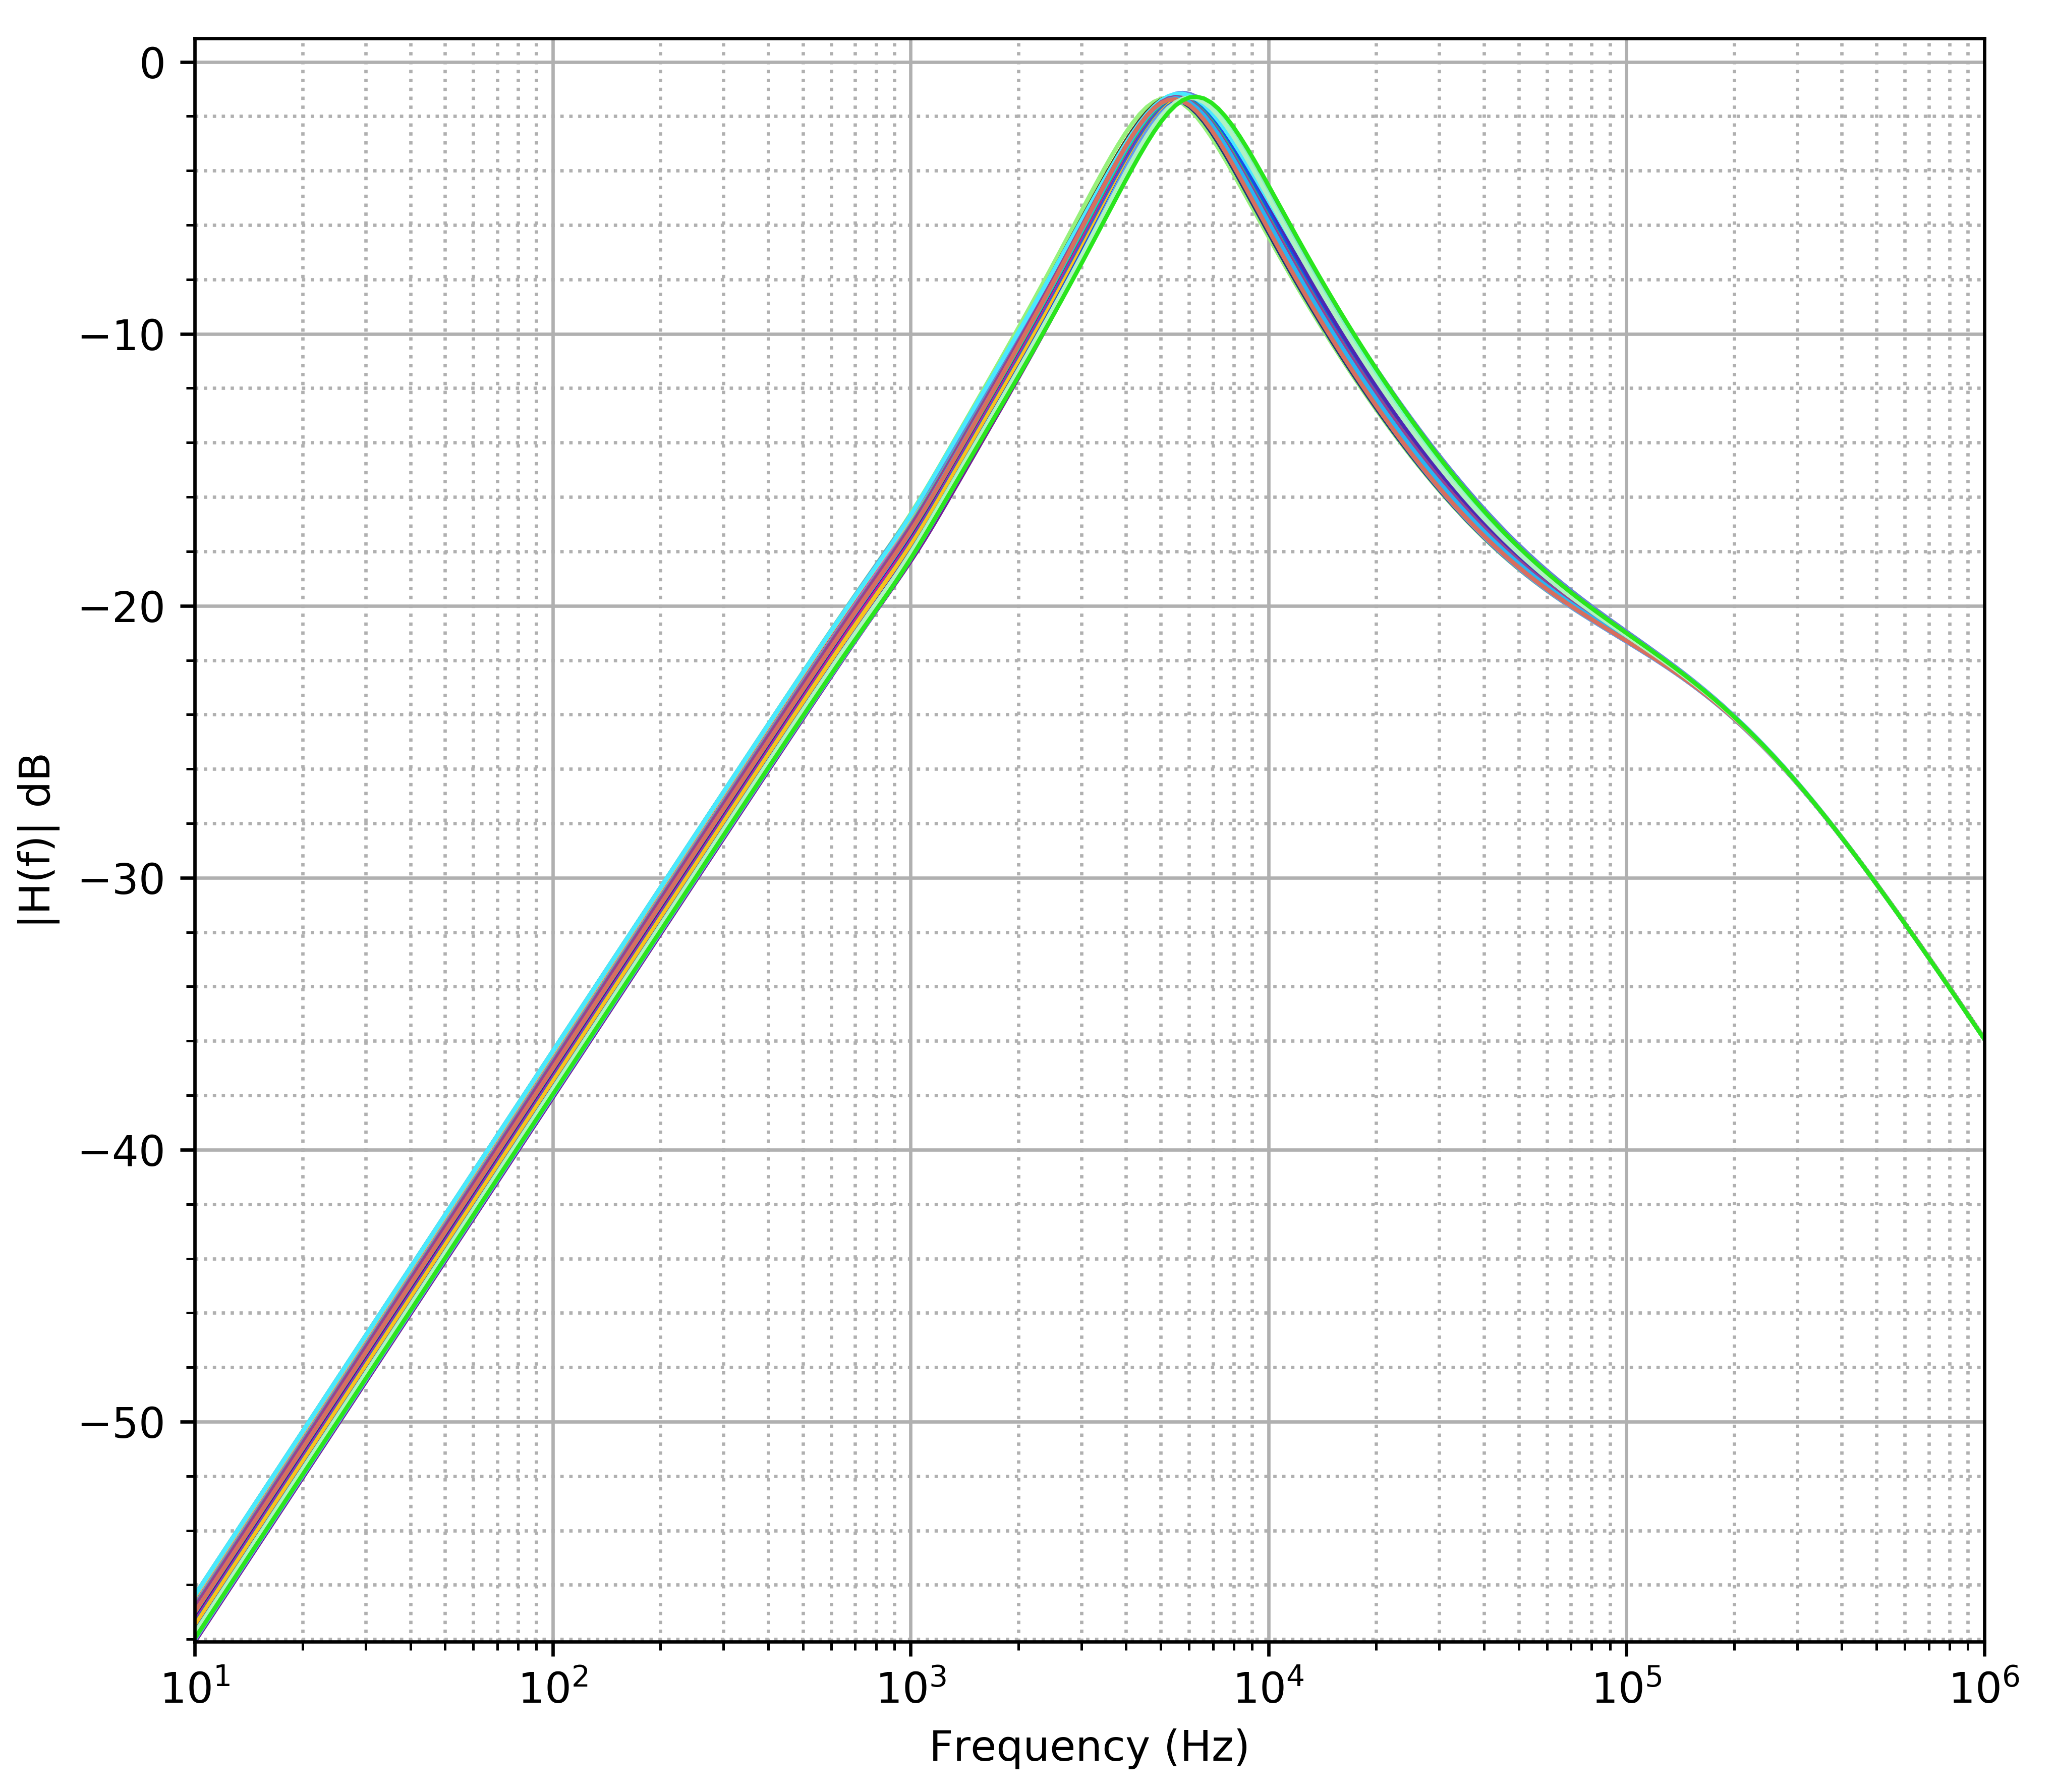
\includegraphics[scale=0.12]{../EJ2/Recursos/bd_montecarlo.png}    
    \caption{Respuesta en frecuencia en m\'odulo del filtro pasabanda}
    \label{fig:bd_montecarlo}
\end{figure}

\begin{figure}[H]
    \centering
        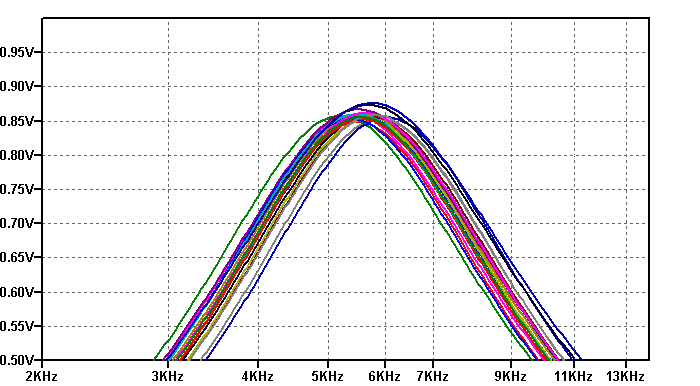
\includegraphics[scale=0.6]{../EJ2/Recursos/bp_montecarlo_frecuencia.png}
    \caption{Acercamiento en escala lineal de la respuesta en frecuencia}
    \label{fig:bp_montecarlo_frecuencia}
\end{figure}

\subsubsection{Resultados}

\subsection{Filtro Rechazabanda}
\subsubsection{Dise\~no de funci\'on transferencia}
Consid\'erese un sistema de segundo orden lineal, de tiempo invariante y bibo-estable, el cual debe caracterizar una respuesta en frecuencia propia de un filtro rechazabanda que aten\'ua todas las frecuencias entorno a una frecuencia determinada,
luego para poder modelizar matem\'aticamente dicho sistema a trav\'es de su funci\'on transferencia se emplea la siguiente ecuaci\'on. Cabe destacar que la expresi\'on ideal de un filtro rechazabanda careza de t\'ermino lineal en el numerador, no obstante
no ser\'a posible alcanzar tal condici\'on en la pr\'actica.

\begin{equation}
    H(s) = \frac{\left( \frac{s}{\omega_o} \right)^{2} + \frac{s}{Q_N \cdot \omega_o} + 1}{\left( \frac{s}{\omega_o} \right)^{2} + \frac{s}{Q_D \cdot \omega_o} + 1}    
\end{equation}

Para completar con este dise\~no del modelo matem\'atico empleado, se imponen como condiciones que la frecuencia de corte del filtro debe encontrarse tal que $\omega_o = 2\pi \cdot f_o =  2\pi \cdot 1kHz$. Adem\'as,
se busca que el numerador tenga un $\xi_N$ lo m\'as chico posible y cercano al valor nulo, mientras que el denominador se busca que tenga un valor lo m\'as cercano a la unidad posible.

\subsubsection{Dise\~no de circuito con Gyrator}
De igual forma que se fue realizando para los circuitos anteriores, se implementa la funci\'on transferencia del filtro rechazabanda replicando como se lo har\'ia con un circuito RLC, donde se busca reemplazar el comportamiento inductivo
por un Gyrator que lo simule, para ello primero se trabajan con equivalente y aproximaciones que permiten el dise\~no r\'apido y simplificado del circuito, posteriormente se analizan las caracter\'isticas no ideales del sistema obtenido y se buscan 
condiciones para maximizar el rango de operaci\'on de estas condiciones ideales.

\paragraph*{Circuito equivalente aproximado:} En la Fig. \ref{fig:equivalente_rechazabanda} se presenta el circuito equivalente de la implementaci\'on a realizar, para este caso se plantea la funci\'on transferencia y se obtiene luego
una funci\'on que se asemeja a la funci\'on deseada. 

\begin{figure}[H]
    \centering
    \includegraphics[scale=0.5]{../EJ2/Recursos/equivalente_rechazabanda.png}
    \caption{Circuito equivalente del rechazabanda}
    \label{fig:equivalente_rechazabanda}
\end{figure}

\begin{equation}
    H(s) = \frac{s^{2} \cdot LC + s \cdot C \cdot R_L + 1}{s^{2} \cdot LC + s \cdot C \cdot (R + R_L) + 1}    
\end{equation}

Entonces se obtiene que la frecuencia de corte del filtro se encuentra en $\omega_o = \frac{1}{\sqrt{LC}} = 2\pi \cdot 1kHz$, adem\'as se buscan los valores de los coeficientes de amortiguamiento tanto del numerador como denominador,
de esta forma se busca que imponiendo valores para los factores de calidad. Vale mencionar que los valores asignados a $Q_D$ y $Q_N$ son arbitrarios, no se posee un requisito espec\'ifico sobre c\'omo debe ser el ancho de banda del filtro.
Entonces, despejando de estas expresiones y buscando valores con el menor error posible, se llega a que $R_L = 100 \Omega$, $R = 1k \Omega$, $C = 100nF$ y $L = 0.2533H$.

\paragraph*{Circuito completo:} En la Fig. \ref{fig:circuito_rechazabanda} se ilustra el circuito completo de la aproximaci\'on considerada, empleando para ello un Gyrator. Al igual que se hizo hasta ahora,
se deben determinar valores para la capacidad $C_2$ y la resistencia $R_2$ para cumplir con el valor de inductancia requerido, adem\'as de con la condici\'on de dise\~no del Gyrator para maximizar el rango de operaci\'on, esto era,
$\omega << \frac{1}{C_2 \cdot R_L}$. Para esto se determina que $C_2 = 8.2nF$ y que $R_2 = 300k\Omega$.

\begin{figure}[H]
    \centering
    \includegraphics[scale=0.6]{../EJ2/Recursos/circuito_rechazabanda.png}
    \caption{Circuito completo del rechazabanda con el Gyrator}
    \label{fig:circuito_rechazabanda}
\end{figure}

\paragraph*{An\'alisis no ideal:} Para el an\'alisis no ideal se considera el amplificador operacional no ideal con un $A_{vol}$ finito con polo dominante, considerando que la impedancia de entrada muy alta con lo cual puede despreciarse la corriente
que circula hacia el interior del amplificador operacional. Se plantean ecuaciones para el circuito y se resuelven para llegar a la expresi\'on final sin aproximar de la funci\'on transferencia.

\begin{align}
    & V^{-} = V_A \\
    & V^{+} = \frac{V_B \cdot s \cdot C_2 \cdot R_2}{1 + s \cdot C_2 \cdot R_2 } \\
    & A_{vol} = \frac{GBP}{s + \omega_p} \\
    & V_A = (V^{+} - V^{-}) \cdot A_{vol} \\
    & I_R = I_{C_2} + I_{R_L} \Rightarrow \frac{V_i - V_B}{R + \frac{1}{s C}} = \frac{V_B}{R_2 + \frac{1}{sC_2}} + \frac{V_B - V_A}{R_L}
\end{align}

Luego, realizando algunos pasos algebraicos dentro de los cuales se encuentra la consideraci\'on de que el $\omega << GBP$ para el rango de frecuencias con las cuales se va a trabajar, entonces
se puede obtener una forma de la transferencia:

\begin{align*}
    &H(s) = \\
    &= \frac{s^{3} \cdot C_2 \cdot R_2 \cdot C^{2} \cdot R \cdot R_L + s^{2} \cdot \left[ C_2 \cdot C \cdot R_L \cdot R_2 \cdot (1 + \frac{R}{R_2}) + C^{2} \cdot R \cdot R_L \right] + s \cdot \left[ C \cdot R \cdot(1 + \frac{R_L}{R}) + C_2 \cdot R_L \right] + 1}{(s^{2} \cdot C_2 \cdot C \cdot R_L \cdot R_2 \cdot (1 + \frac{R}{R_2}) + s \cdot C \cdot R \cdot ( 1 + \frac{R_L}{R}) + s \cdot C_2 \cdot R_L + 1) \cdot (s \cdot C \cdot R + 1)}
\end{align*}

Considerando que $R_2 >> R$, $R >> R_L$, $\omega << \frac{1}{C_2 \cdot C_L}$, y que adem\'as $R \cdot C << R_2 \cdot C_2$, luego como consecuencia de ello pueden despreciar algunos t\'erminos reescribiendo adecuadamente la funci\'on transferencia,
obteniendo una forma aproximada que se asemeja a la forma aproximada del circuito equivalente empleado previamente para el dise\~no. Entonces:

\begin{equation}
    H(s) \approx \frac{s^{2} \cdot C_2 \cdot C \cdot R_L \cdot R_2 + s \cdot C \cdot R_L + 1}{s^{2} \cdot C \cdot C_2 \cdot R_L \cdot R_2 + s \cdot C \cdot (R + R_L) + 1}
\end{equation}

\subsubsection{Verificaci\'on del dise\~no}
Se realiza la simulaci\'on del circuito en LTSpice con un an\'alisis de Monte Carlo para considerar la dispersi\'on del valor de los componentes en la realidad.
Los resultados se pueden observar en las figuras \ref{fig:br_montecarlo} y \ref{fig:br_montecarlo_frecuencia}.

\begin{figure}[H]
    \centering
        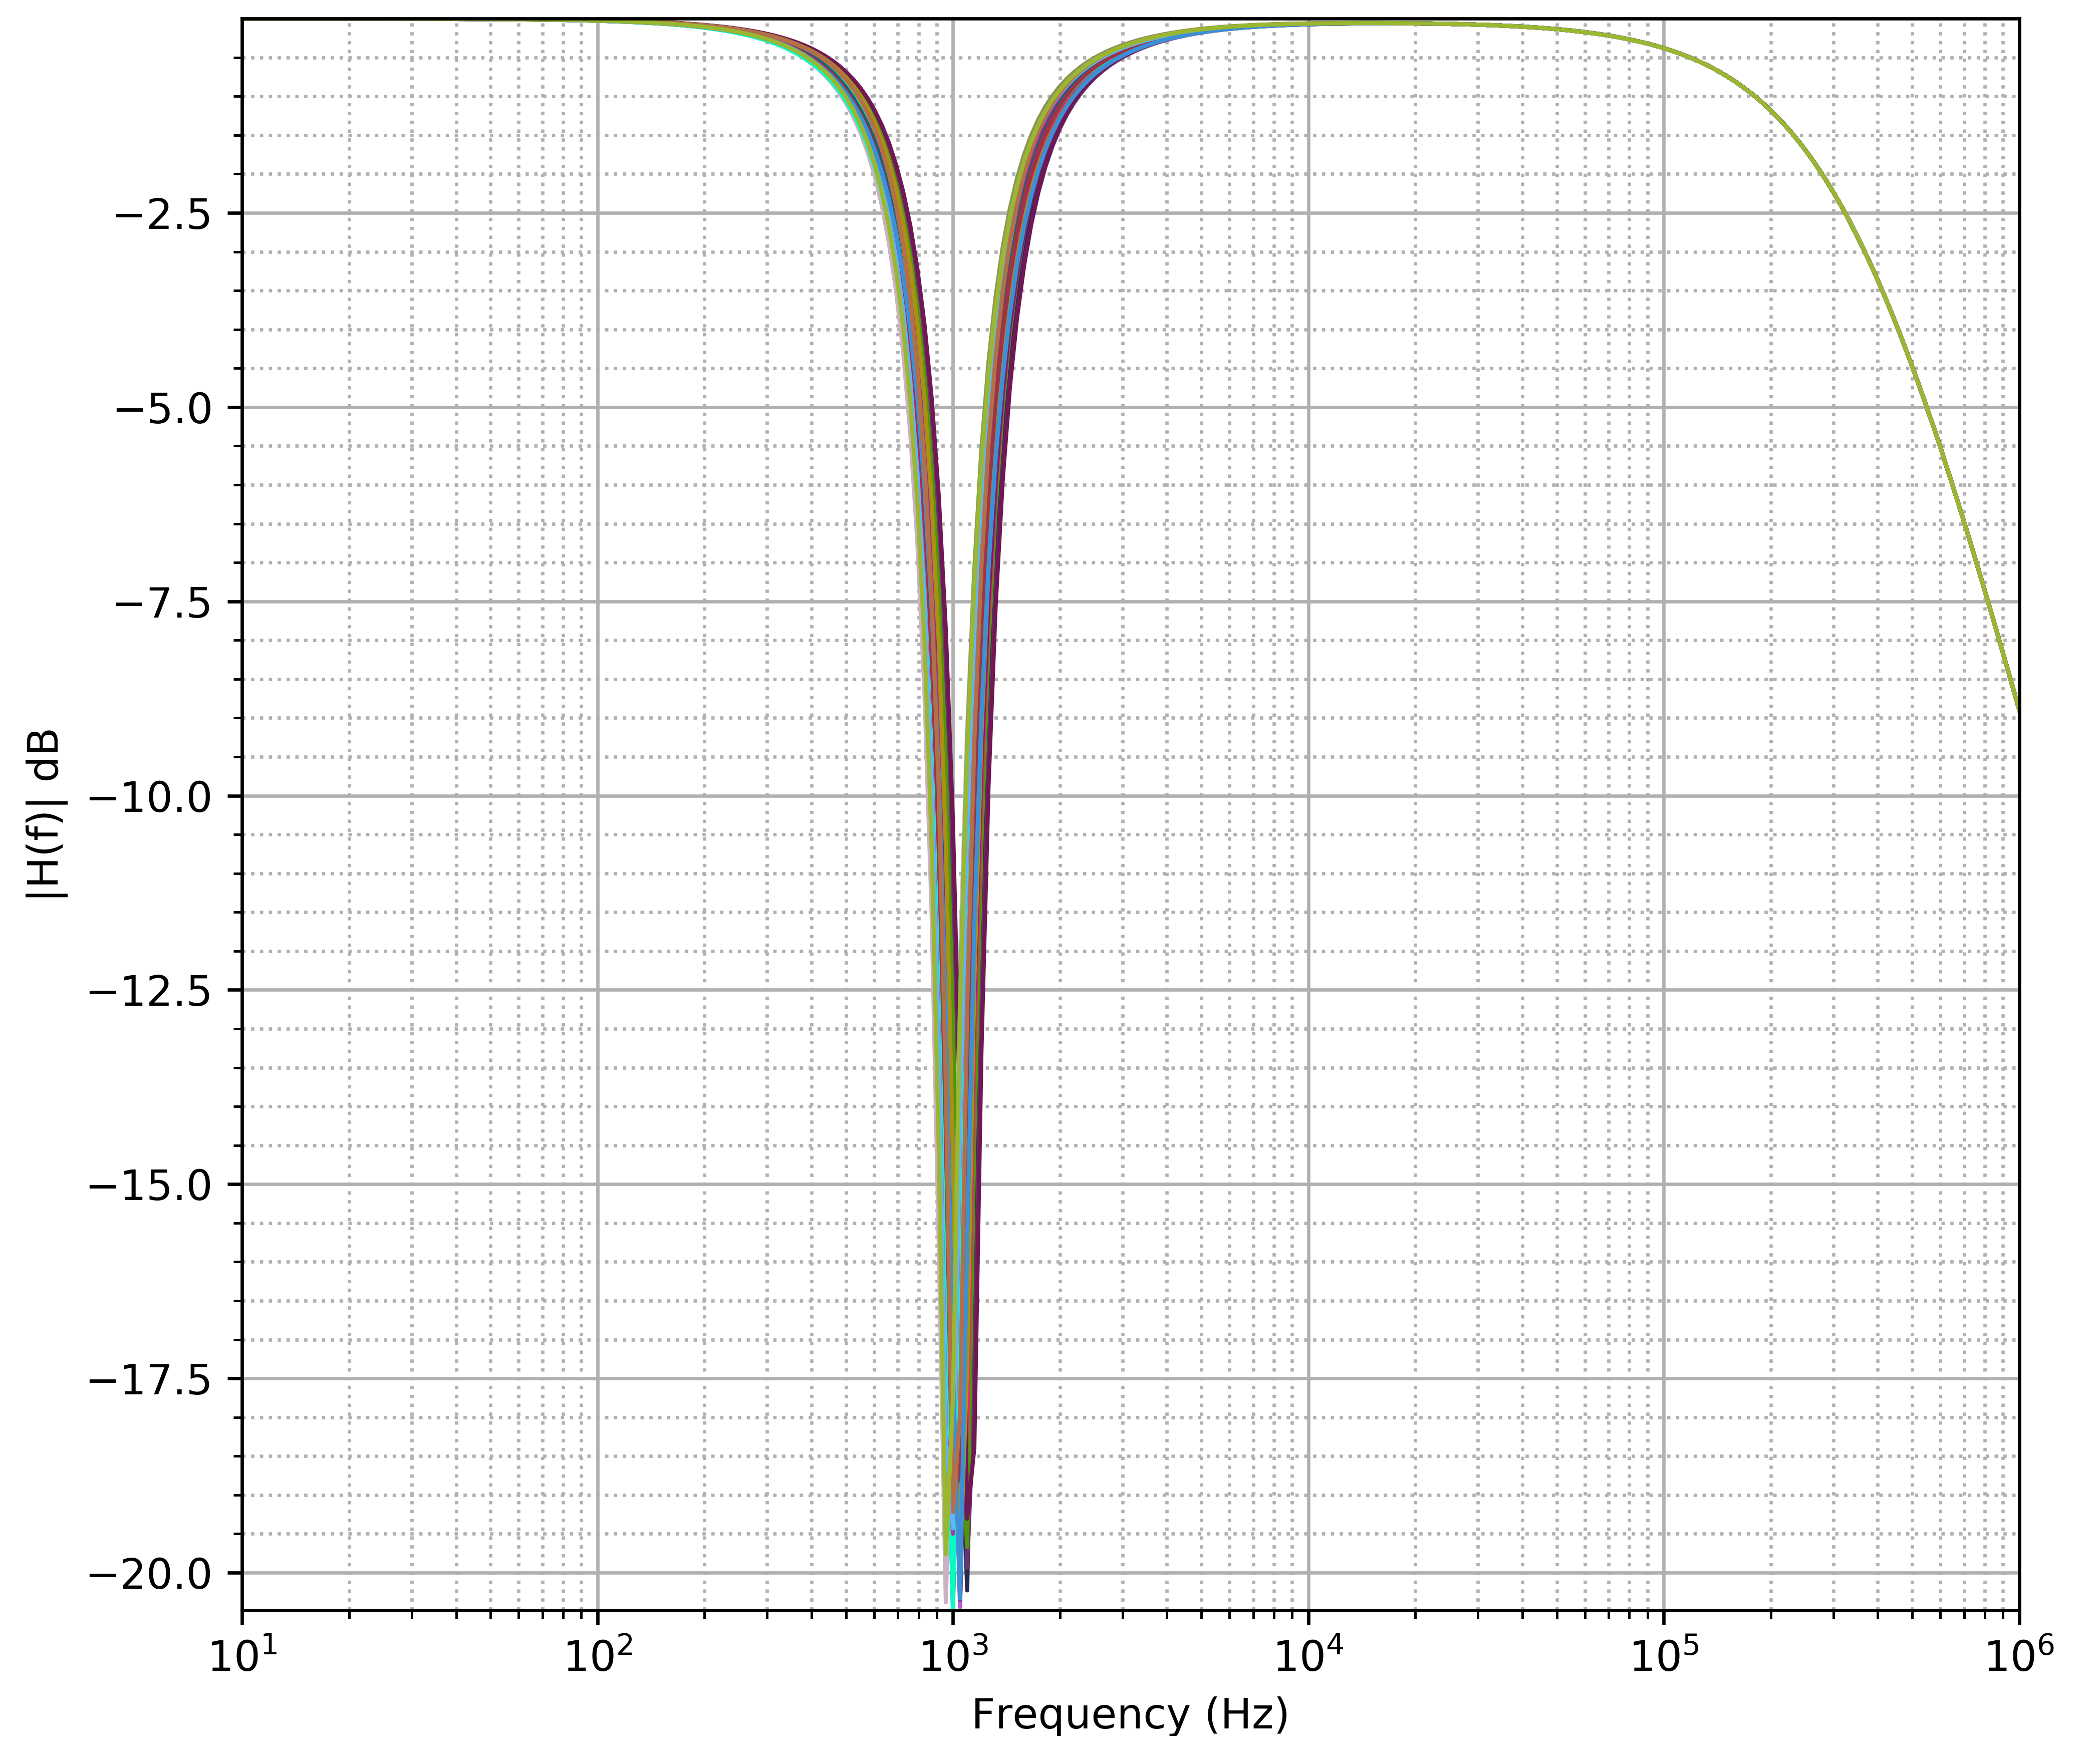
\includegraphics[scale=0.12]{../EJ2/Recursos/br_montecarlo.png}
    \caption{Respuesta en frecuencia en m\'odulo del filtro rechazabanda}
    \label{fig:br_montecarlo}
\end{figure}

\begin{figure}[H]
    \centering
    \begin{tabular}{c c}
        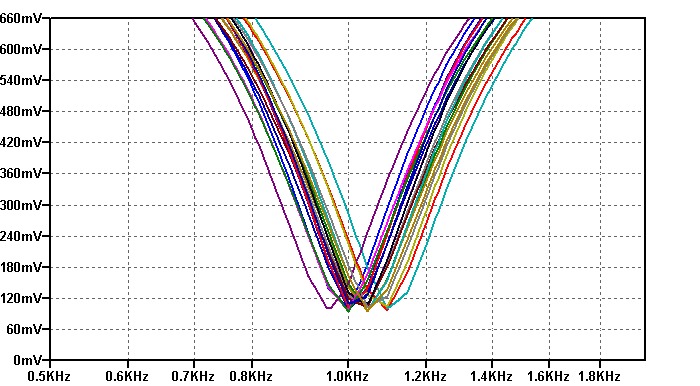
\includegraphics[scale=0.6]{../EJ2/Recursos/br_montecarlo_frecuencia.png}
    \end{tabular}
    \caption{Acercamiento a la frecuencia del filtro rechazabanda}
    \label{fig:br_montecarlo_frecuencia}
\end{figure}

\subsubsection{Resultados}

\subsection{Implementaci\'on pr\'actica}
\subsubsection{Selecci\'on del amplificador operacional}
\subsubsection{Esquem\'atico del circuito}
\subsubsection{Dise\~no del PCB y vista 3D}
